% ============================================
% FULL PAPER - A Multi-Layer Machine Learning Framework 
% for DDoS Detection in IoT Networks with Adaptive Decision Engine
% ============================================

\documentclass[conference]{IEEEtran}
\IEEEoverridecommandlockouts

% Packages
\usepackage{cite}
\usepackage{amsmath,amssymb,amsfonts}
\usepackage{algorithmic}
\usepackage{graphicx}
\usepackage{textcomp}
\usepackage{xcolor}
\usepackage{booktabs}
\usepackage{multirow}
\usepackage{url}

\begin{document}

\title{A Multi-Layer Machine Learning Framework for DDoS Detection in IoT Networks with Adaptive Decision Engine}

\author{\IEEEauthorblockN{Nguyen Tat Thang, Tran Dang Cong}
\IEEEauthorblockA{Faculty of Information Technology, Dai Nam University, Ha Noi\\
Email: congtd@dainam.edu.vn}}

\maketitle

\begin{abstract}
The rapid proliferation of Internet of Things (IoT) devices has significantly increased the attack surface of modern network infrastructures, making Distributed Denial-of-Service (DDoS) attacks a critical security concern. This paper proposes a multi-layer machine learning framework for intelligent DDoS detection in IoT networks, integrating protocol-level analysis and network traffic analytics with an adaptive decision engine. The proposed framework performs intrusion detection on both MQTT communication traffic and general network flows using benchmark datasets. To address severe class imbalance, data preprocessing techniques such as feature encoding, normalization, SMOTE, and random under-sampling are employed. Four machine learning algorithms are evaluated: Decision Tree, Random Forest, LightGBM, and XGBoost. LightGBM achieves the best performance for MQTT traffic (F1-score: 91.26\%), while XGBoost excels for network traffic (F1-score: 90.28\%). Furthermore, an adaptive decision engine incorporating Isotonic Calibration and Attack Bias Logic significantly improves detection performance, achieving final F1-scores of 93.06\% for MQTT traffic and 95.23\% for network traffic. The system demonstrates low inference latency suitable for real-time deployment.
\end{abstract}

\begin{IEEEkeywords}
DDoS detection, Multi-layer machine learning, IoT network security
\end{IEEEkeywords}

\section{Introduction}

\subsection{Background and Motivation}


The Internet of Things (IoT) has revolutionized modern computing by connecting billions of devices worldwide, enabling smart homes, industrial automation, healthcare monitoring, and intelligent transportation systems. However, this rapid expansion has created significant security vulnerabilities. IoT devices often have limited computational resources, weak authentication mechanisms, and inadequate security updates, making them attractive targets for cyber attackers \cite{iot_security}.

Distributed Denial-of-Service (DDoS) attacks represent one of the most severe threats to IoT networks. In a DDoS attack, multiple compromised devices flood a target system with excessive traffic, overwhelming its resources and rendering services unavailable to legitimate users. The Mirai botnet attack in 2016, which compromised over 600,000 IoT devices, demonstrated the devastating potential of IoT-based DDoS attacks \cite{mirai_attack}.

Traditional security mechanisms, such as signature-based intrusion detection systems, struggle to detect sophisticated DDoS attacks in IoT environments. These methods rely on predefined attack patterns and cannot adapt to evolving attack strategies. Moreover, the heterogeneous nature of IoT networks, which includes diverse protocols like MQTT (Message Queuing Telemetry Transport), requires specialized detection approaches for different communication layers.

\subsection{Research Gap and Motivation}

Recent research has explored machine learning approaches for network intrusion detection. However, several critical gaps remain:

\textbf{Limited Protocol Coverage:} Most existing studies focus on either network-level traffic analysis or application-level protocol detection, but rarely integrate both. MQTT requires specialized analysis due to its unique communication patterns.

\textbf{Class Imbalance Problem:} Real-world network traffic datasets exhibit severe class imbalance, where normal traffic significantly outnumbers attack traffic. This imbalance causes machine learning models to bias toward the majority class.

\textbf{Lack of Adaptive Decision Mechanisms:} Existing detection systems typically output binary classifications without considering prediction confidence or threat severity.

\subsection{Research Objectives and Contributions}

This paper addresses these gaps by proposing a comprehensive multi-layer machine learning framework for DDoS detection in IoT networks. The main contributions include:

\begin{enumerate}
\item \textbf{Multi-Layer Detection Framework:} A novel architecture combining MQTT protocol-level analysis with network traffic analysis.

\item \textbf{Advanced Preprocessing Pipeline:} Systematic preprocessing using feature encoding, normalization, SMOTE over-sampling, and random under-sampling.

\item \textbf{Comprehensive Algorithm Evaluation:} Systematic comparison of four machine learning algorithms with detailed performance analysis.

\item \textbf{Adaptive Decision Engine:} An intelligent decision mechanism incorporating Isotonic Calibration and Attack Bias Logic, improving F1-scores by 1.80\% for MQTT and 4.95\% for network traffic.
\end{enumerate}


\subsection{Paper Organization}

The remainder of this paper is organized as follows: Section II reviews related work and theoretical foundations. Section III presents the proposed methodology. Section IV discusses experimental results. Section V provides recommendations and concludes the paper.

\section{Literature Review}

\subsection{DDoS Attacks in IoT Networks}

DDoS attacks can be categorized into volumetric attacks, protocol attacks, and application-layer attacks \cite{ddos_taxonomy}. IoT networks face unique vulnerabilities due to device constraints. The MQTT protocol, while efficient for IoT communication, introduces additional security concerns.

\subsection{Machine Learning for Intrusion Detection}

Machine learning has emerged as a powerful approach for network intrusion detection. Random Forest provides robust baseline performance through ensemble learning \cite{random_forest}. XGBoost uses regularization to prevent overfitting and supports parallel processing \cite{xgboost}. LightGBM employs histogram-based learning for faster training \cite{lightgbm}.

\subsection{Class Imbalance Handling}

SMOTE addresses class imbalance by generating synthetic samples for minority classes through interpolation \cite{smote}. Random under-sampling reduces the majority class. Hybrid approaches combine both techniques effectively.

\subsection{Probability Calibration}

Isotonic Regression is a non-parametric calibration method that maps predicted probabilities to calibrated probabilities \cite{isotonic_calibration}. This is essential for security applications where decision confidence affects response strategies.

\section{Research Methodology}

\subsection{Overall Framework Architecture}

Our proposed framework consists of four sequential phases:

\begin{enumerate}
\item Data Preprocessing
\item Model Training and Comparison
\item Model Optimization
\item Adaptive Decision Engine
\end{enumerate}

The framework operates on two parallel layers: MQTT protocol layer and network traffic layer, with each layer following the same four-phase pipeline.


\subsection{Phase 1: Data Preprocessing}

Data preprocessing is a critical foundation for machine learning model performance. Our preprocessing pipeline systematically transforms raw network traffic data into a standardized format suitable for model training, addressing challenges including missing values, categorical feature encoding, feature scaling, and data format consistency.

\subsubsection{MQTT Traffic Preprocessing}

We utilize the MQTT IoT Intrusion Detection Dataset, which contains network traffic captured from MQTT-based IoT devices under various attack scenarios. MQTT (Message Queuing Telemetry Transport) is a lightweight publish-subscribe messaging protocol widely adopted in IoT applications due to its low bandwidth requirements and efficient message delivery. The dataset comprises 231,646 training samples and 99,290 testing samples, each with 42 features representing protocol-specific metrics, network flow characteristics, and statistical properties that capture both normal communication patterns and various attack behaviors.

The dataset exhibits severe class imbalance, a common challenge in security applications where normal traffic vastly outnumbers malicious activities. The distribution of traffic types in the training set is as follows: legitimate traffic (50.0\%, 115,824 samples) representing normal IoT device communication, dos attacks (39.3\%, 91,156 samples) attempting to exhaust system resources, bruteforce attacks (4.4\%, 10,150 samples) trying multiple password combinations, malformed packets (3.3\%, 7,646 samples) with corrupted protocol structures, slowite attacks (2.8\%, 6,441 samples) maintaining prolonged connections to consume resources, and flood attacks (0.2\%, 429 samples) overwhelming the network with excessive traffic. The extreme rarity of flood attacks, comprising only 0.2\% of samples, presents a significant challenge for model training and necessitates specialized handling techniques in subsequent phases.

The preprocessing pipeline consists of eight systematic steps designed to ensure data quality and consistency. First, we load the pre-split training (70\%) and testing (30\%) datasets, which ensures consistent evaluation across experiments and prevents data leakage. This split ratio balances the need for sufficient training data while maintaining adequate test samples for reliable performance assessment. Second, we conduct comprehensive examination of the dataset to identify missing, null, or undefined values, as missing data can significantly impact model performance by introducing bias or reducing statistical power. Our analysis reveals no missing values in the MQTT dataset, eliminating the need for imputation techniques. Third, we separate independent variables (features) from the dependent variable (label), where the feature matrix X contains all 42 network traffic characteristics, while the label vector y contains attack type classifications.

Fourth, we systematically identify features with categorical (non-numerical) values that require encoding. In the MQTT dataset, categorical features include protocol type (TCP, UDP, ICMP), service type (HTTP, MQTT, DNS), connection state (established, closed, time-wait), and MQTT-specific attributes such as message type and quality of service level. These categorical variables cannot be directly processed by machine learning algorithms and must be converted to numerical representations. Fifth, we apply Label Encoding to convert categorical features into numerical representations, where each unique category is assigned an integer value. For example, protocol types might be encoded as TCP=0, UDP=1, ICMP=2. This transformation preserves the categorical nature of the data while making it computationally tractable. We carefully track the encoding mappings to ensure consistent transformation of new data during deployment.

Sixth, we apply StandardScaler to normalize numerical features, transforming them to have zero mean and unit variance using the formula z = (x - μ) / σ, where x is the original value, μ is the mean, and σ is the standard deviation. This standardization is crucial because features in network traffic data have vastly different scales. For instance, packet counts might range from 1 to 10,000, while duration might range from 0.001 to 100 seconds, and byte counts could reach millions. Without scaling, features with larger magnitudes would dominate the learning process, causing the model to overlook important patterns in smaller-scale features. StandardScaler computes the mean and standard deviation for each feature from the training data, then transforms both training and test data using these statistics, ensuring consistent scaling across datasets.

Seventh, we save the fitted encoders and scaler as preprocessing artifacts in serialized format. These artifacts are essential for maintaining consistency between training and deployment. When the trained model is deployed to process new network traffic in real-time, incoming data must undergo identical preprocessing transformations using the exact same encoding mappings and scaling parameters learned from the training data. Without preserving these artifacts, the model would receive inconsistently preprocessed data, leading to degraded performance or complete failure. Eighth, we export the preprocessed training and testing datasets in a standardized format for subsequent phases, with the exported data maintaining the transformed feature values, encoded categorical variables, and scaled numerical features, ready for immediate use in model training without requiring additional preprocessing steps.

Figure \ref{fig:mqtt_label_dist} shows the severe class imbalance in the MQTT dataset, clearly illustrating the challenge that must be addressed in the training phase.

\begin{figure}[htbp]
\centerline{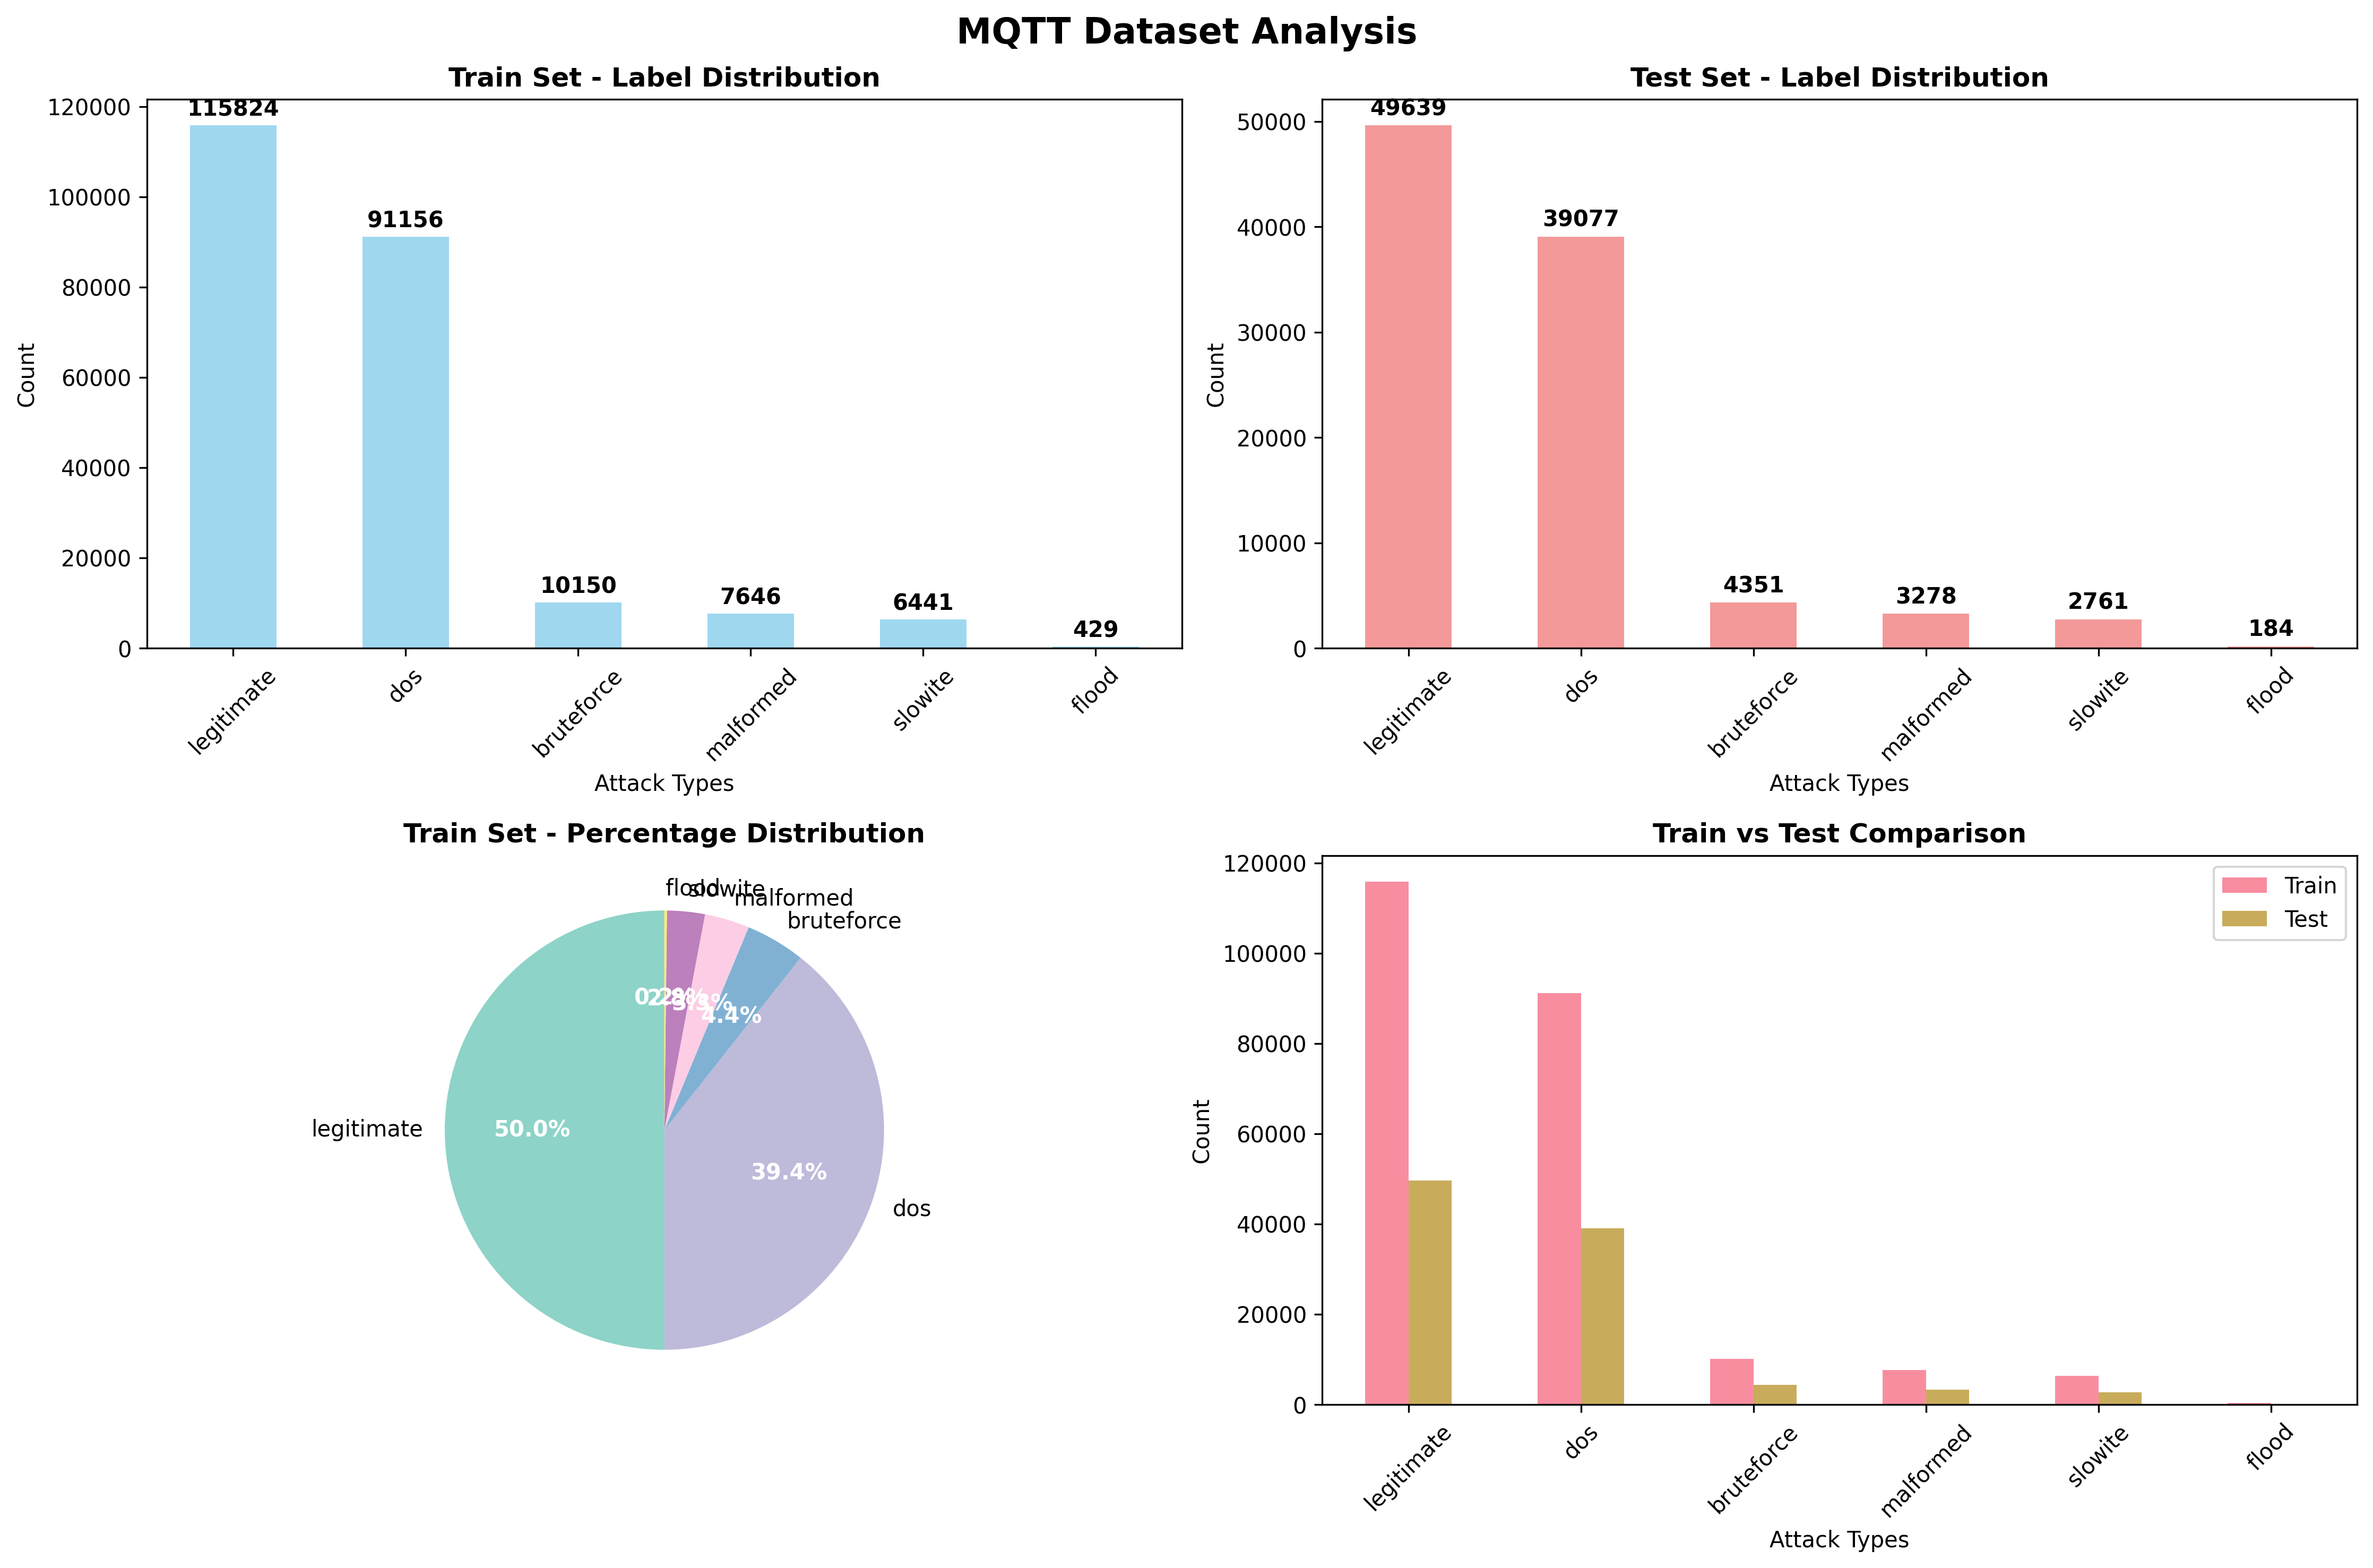
\includegraphics[width=0.48\textwidth]{Images/Phase1_MQTT_label_distribution.png}}
\caption{MQTT Dataset Label Distribution showing severe class imbalance with flood attacks comprising only 0.2\% of samples}
\label{fig:mqtt_label_dist}
\end{figure}

\subsubsection{Network Traffic Preprocessing}

For network-level detection, we employ the UNSW-NB15 dataset, a comprehensive benchmark containing modern network attack types that reflect contemporary cyber threats. This dataset was created by the Australian Centre for Cyber Security and includes both normal network activities and nine categories of modern attack behaviors. The dataset contains 42 features representing network flow characteristics such as connection duration, protocol information, service types, packet counts in both directions, byte counts, TCP window sizes, and various statistical metrics computed from network flows.

The preprocessing pipeline for network traffic follows the same eight-step systematic process as MQTT preprocessing, ensuring consistency in our methodology. However, the network dataset presents different characteristics and challenges. The label distribution shows approximately 87\% normal traffic and 13\% attack traffic, reflecting realistic network conditions where legitimate traffic vastly outnumbers malicious activities. The attack categories include various modern threats: DoS and DDoS attacks, Exploits targeting system vulnerabilities, Fuzzers attempting to discover security flaws, Generic attacks using common attack patterns, Reconnaissance activities for information gathering, Shellcode injection attempts, Worms for self-propagating malware, and Backdoor installations for persistent access. After preprocessing, we obtain standardized datasets with encoded categorical features and normalized numerical features, ready for model training with preprocessing artifacts preserved to ensure consistent transformation of new data during model deployment and real-time detection operations.

\subsection{Phase 2: Model Training and Comparison}

Phase 2 focuses on training and systematically comparing multiple machine learning algorithms to identify the most effective approach for each traffic type. This phase addresses the severe class imbalance problem through advanced resampling techniques and evaluates four state-of-the-art algorithms using comprehensive performance metrics.

\subsubsection{Class Imbalance Handling}

The severe class imbalance observed in both datasets presents a fundamental challenge for machine learning classification. In imbalanced datasets, standard training procedures cause models to develop a strong bias toward the majority class, as correctly predicting the majority class yields high overall accuracy even when minority classes are completely ignored. This bias is particularly problematic in security applications where the minority classes (attacks) are precisely the events we need to detect reliably.

To address this challenge, we implement a sophisticated hybrid resampling approach that combines two complementary techniques: Synthetic Minority Over-sampling Technique (SMOTE) for minority class augmentation and random under-sampling for majority class reduction.

SMOTE operates by selecting a minority class sample, identifying its five nearest neighbors in the feature space using Euclidean distance, randomly choosing one of these neighbors, and creating a new synthetic sample by interpolating between the original sample and the selected neighbor. The interpolation is performed along the line segment connecting the two samples, with the new sample placed at a random point along this line. This process effectively increases minority class representation while maintaining the underlying distribution characteristics of the original data. Unlike simple duplication, SMOTE creates diverse synthetic samples that help the model learn more robust decision boundaries. For our implementation, we use k=5 nearest neighbors, which provides a good balance between generating diverse samples and maintaining the local structure of the minority class distribution.

Simultaneously, we reduce the majority class by randomly removing samples until achieving a more balanced distribution. The target distribution aims for approximately equal representation across classes, though exact balance may not be optimal for all scenarios. Under-sampling reduces computational requirements and prevents the model from being overwhelmed by majority class examples. However, we carefully monitor this process to ensure that important patterns in the majority class are not lost through excessive removal.

The hybrid approach combines the strengths of both techniques: SMOTE enriches minority class representation with diverse synthetic samples, while under-sampling prevents majority class dominance without requiring excessive synthetic sample generation. This balanced dataset enables classifiers to learn patterns from all classes effectively, rather than biasing toward the majority class. Critically, this resampling is applied only to training data. The test data remains in its original, naturally imbalanced distribution to evaluate real-world performance. This evaluation strategy ensures that our performance metrics reflect how the model will perform when deployed in actual network environments where attack traffic is naturally rare.


\subsubsection{Machine Learning Algorithms}

We evaluate four state-of-the-art machine learning algorithms, each representing different approaches to ensemble learning and offering distinct advantages for intrusion detection. The systematic comparison of these algorithms enables us to identify the most suitable approach for each traffic type based on empirical performance rather than theoretical assumptions.

\textbf{Decision Tree:} Decision Tree is a fundamental machine learning algorithm that creates a tree-like model of decisions based on feature values. At each internal node, the tree splits the data based on a feature threshold that maximizes information gain or minimizes impurity. The tree continues growing until reaching leaf nodes that represent class predictions. We configure Decision Tree with maximum depth of 20 to prevent excessive tree growth that could lead to overfitting, and minimum samples split of 5 to ensure sufficient data at each node before allowing a split. We also employ class weighting to handle the remaining imbalance after SMOTE and under-sampling. While Decision Trees provide interpretable rules and fast prediction times, they are prone to overfitting and may not capture complex patterns as effectively as ensemble methods.

\textbf{Random Forest:} Random Forest is an ensemble method that constructs multiple decision trees during training and outputs the mode (most common prediction) of their individual predictions for classification tasks. Each tree is trained on a random subset of the training data through bootstrap sampling (sampling with replacement), and at each split point, only a random subset of features is considered. This dual randomization in both samples and features reduces overfitting and improves generalization compared to single decision trees. We configure Random Forest with 100 estimators (individual trees) to provide sufficient ensemble diversity, maximum depth of 20 to control individual tree complexity, and class weighting to handle imbalanced data. The algorithm runs in parallel across multiple CPU cores (n\_jobs=-1), significantly reducing training time. Random Forest typically provides robust baseline performance and good resistance to overfitting, making it a popular choice for many classification tasks.

\textbf{LightGBM (Light Gradient Boosting Machine):} LightGBM is a histogram-based gradient boosting framework developed by Microsoft that achieves faster training speed and lower memory usage compared to traditional gradient boosting implementations. Unlike Random Forest's parallel tree construction, LightGBM builds trees sequentially, with each new tree attempting to correct the errors made by previous trees. LightGBM uses two key innovations: histogram-based learning that bins continuous features into discrete bins (typically 255 bins), reducing computational complexity from O(data × features) to O(bins × features), and leaf-wise tree growth strategy that splits the leaf with maximum loss reduction rather than growing trees level-wise. This approach can achieve better accuracy with fewer trees but requires careful tuning to prevent overfitting. We configure LightGBM with 100 estimators, learning rate of 0.1 to control the contribution of each tree, 31 leaves per tree, and class weighting for imbalanced data. The learning rate acts as a shrinkage parameter, making the boosting process more conservative and improving generalization. LightGBM's efficiency makes it particularly suitable for large datasets and scenarios requiring frequent model updates.

\textbf{XGBoost (eXtreme Gradient Boosting):} XGBoost is an optimized implementation of gradient boosting that has become one of the most popular machine learning algorithms due to its strong performance across diverse tasks. Like LightGBM, XGBoost builds trees sequentially, but it uses a level-wise tree growth strategy that grows all nodes at the same depth before moving to the next level. XGBoost incorporates L1 (Lasso) and L2 (Ridge) regularization terms in its objective function to prevent overfitting, supports parallel processing for faster training despite sequential tree building through parallelized tree construction, and handles missing values automatically by learning the best direction for missing values at each split. We configure XGBoost with 100 estimators, learning rate of 0.1, maximum depth of 20, and scale\_pos\_weight parameter to handle class imbalance. For network traffic detection, we utilize GPU acceleration (device='cuda') to further speed up training. XGBoost's combination of regularization, parallel processing, and robust handling of various data characteristics makes it highly effective for complex classification tasks.

Each algorithm is trained on the balanced training dataset created through our hybrid resampling approach and evaluated on the original (unbalanced) test dataset. This evaluation strategy is crucial as it reflects real-world deployment scenarios where attack traffic is naturally rare compared to normal traffic. Training on balanced data helps the model learn patterns from all classes, while testing on imbalanced data assesses how well the model performs in realistic conditions. We employ multiple evaluation metrics to assess model performance comprehensively: Accuracy measures overall correctness, Precision calculates the proportion of true positive predictions among all positive predictions (minimizing false alarms), Recall measures the proportion of actual positive cases correctly identified (minimizing missed attacks), F1-score computes the harmonic mean of precision and recall (balancing both concerns), and Training Time measures computational efficiency. For multi-class classification (MQTT traffic), we report macro-averaged metrics that treat all classes equally. For binary classification (network traffic), we focus on attack detection performance.

Figure \ref{fig:mqtt_model_comparison} shows the comprehensive performance comparison for MQTT traffic detection across all four algorithms.

\begin{figure}[htbp]
\centerline{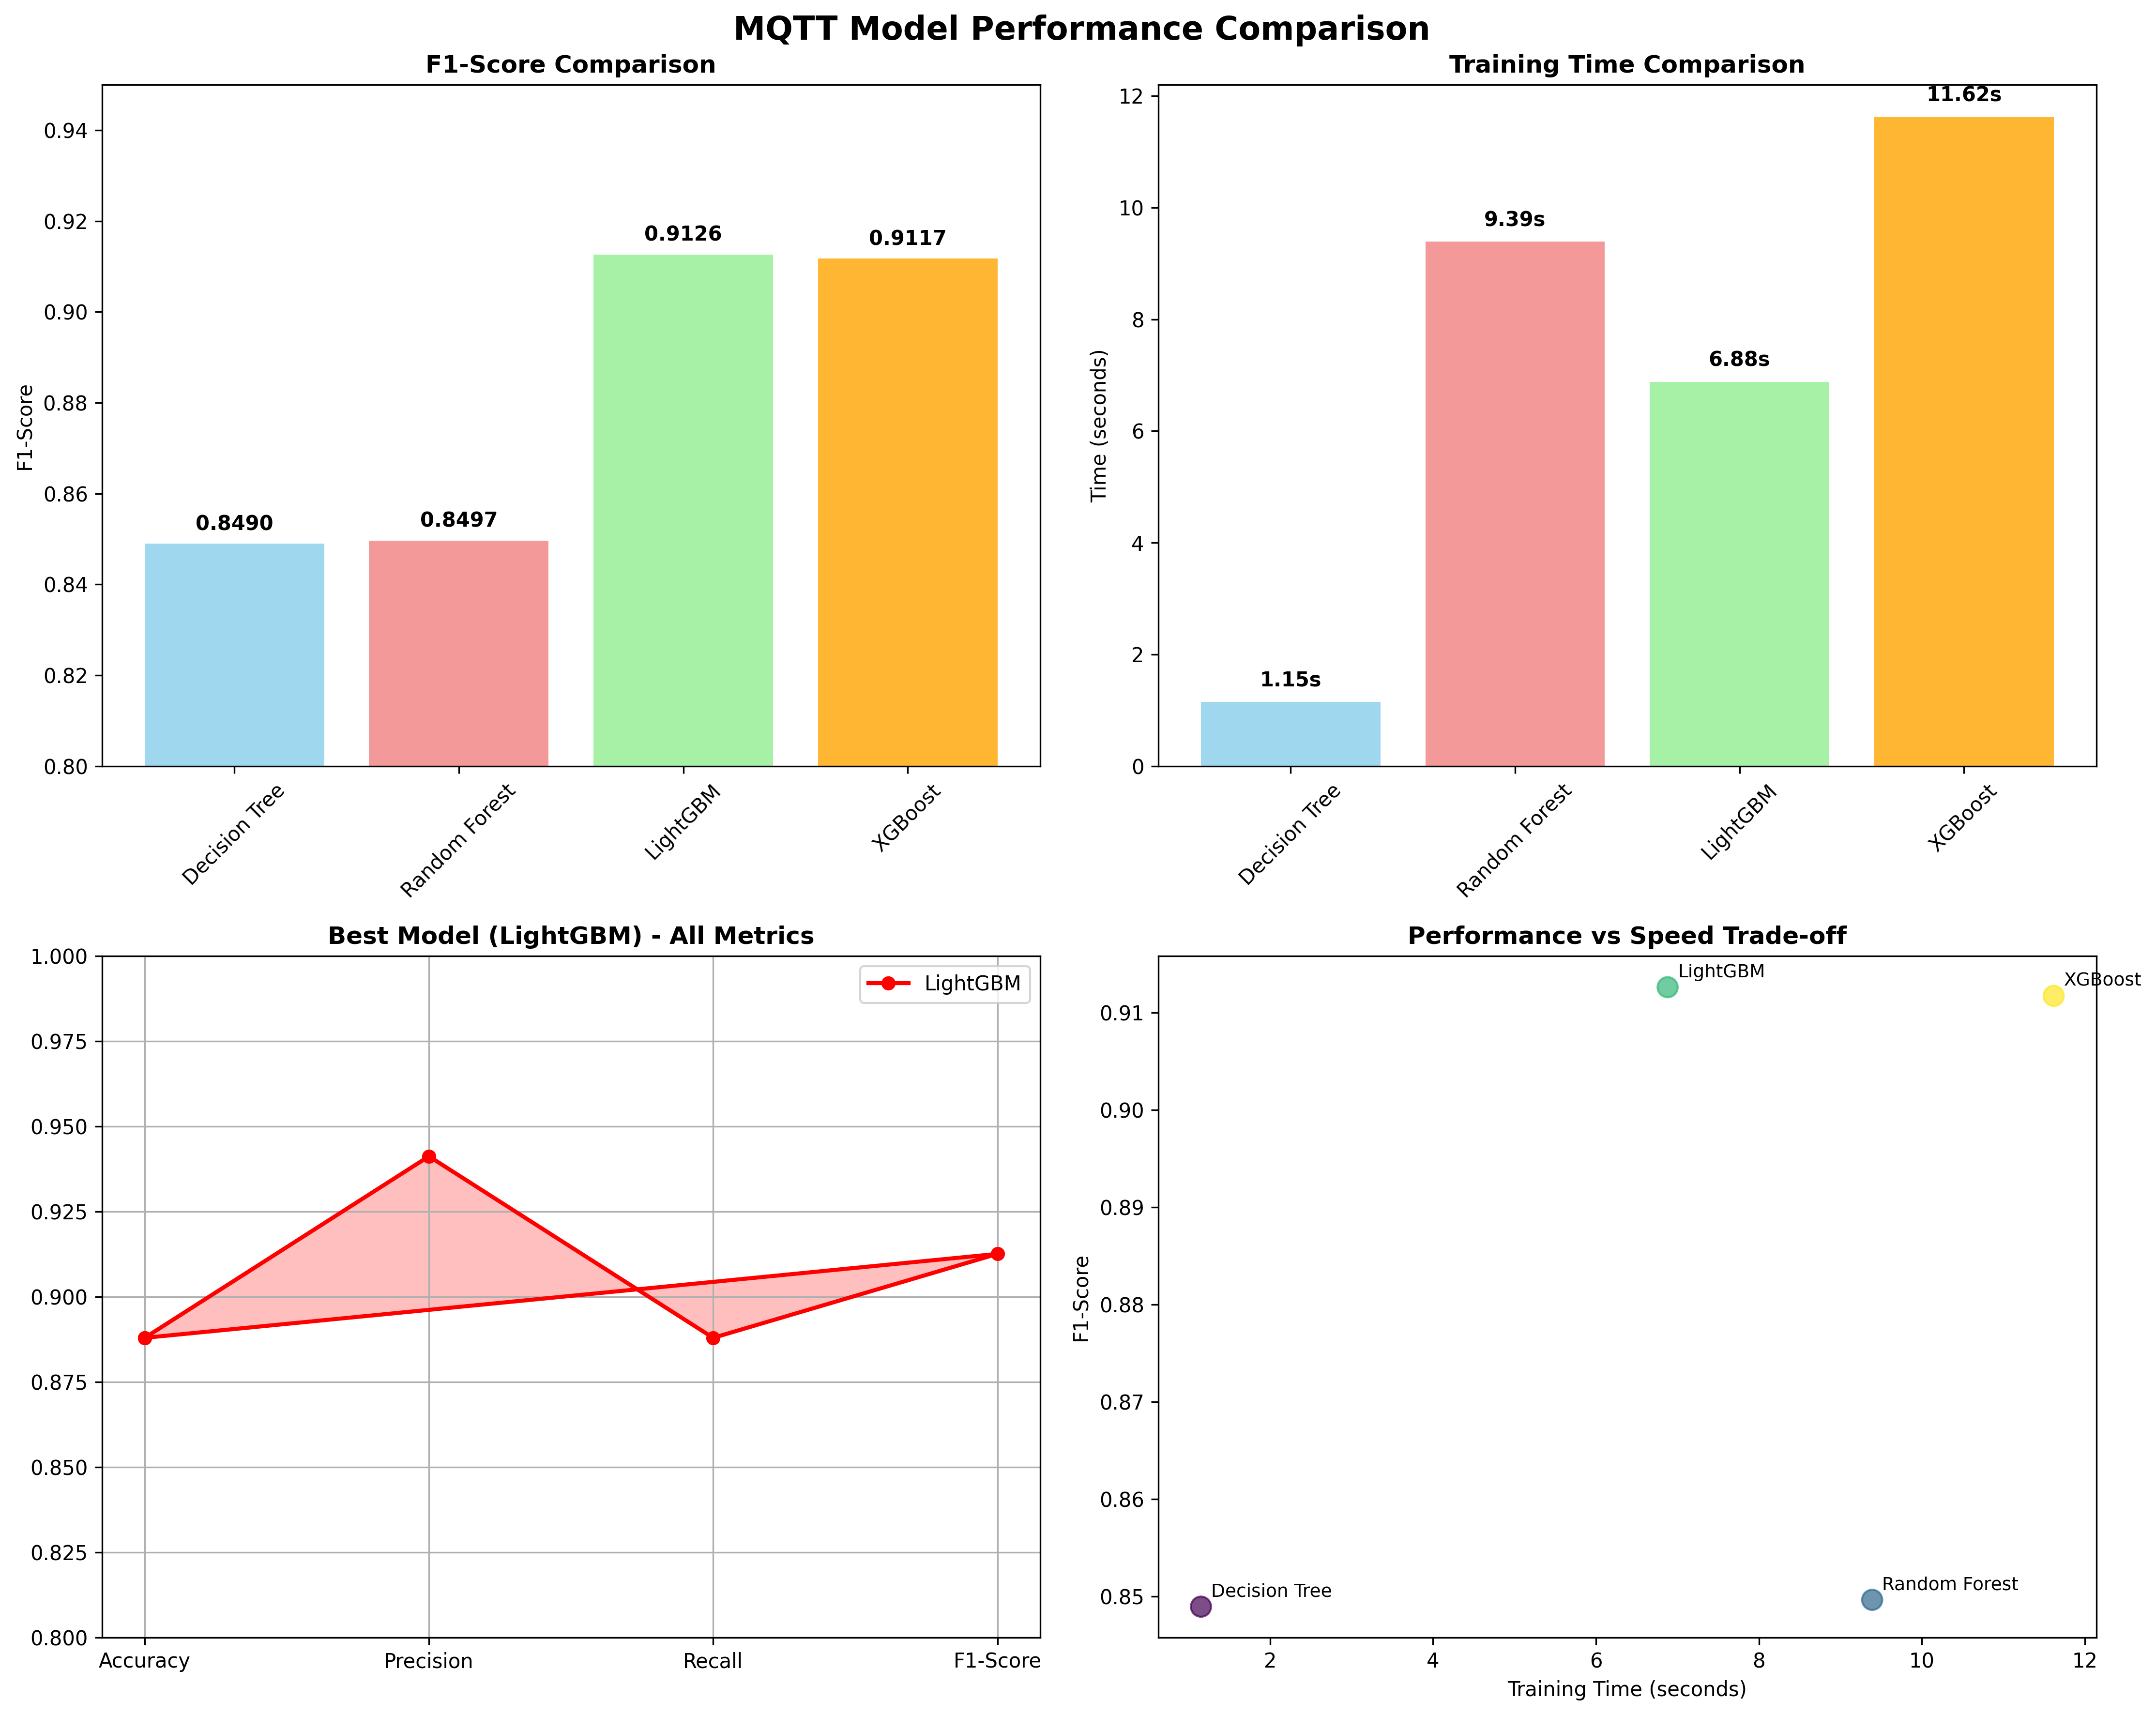
\includegraphics[width=0.48\textwidth]{Images/Phase2_MQTT_model_comparison.png}}
\caption{Model Performance Comparison for MQTT Traffic Detection showing LightGBM achieving the best F1-score of 91.26\%}
\label{fig:mqtt_model_comparison}
\end{figure}

\subsection{Phase 3: Model Optimization}

Phase 3 focuses on fine-tuning the best-performing models identified in Phase 2 through systematic hyperparameter optimization. Hyperparameters are configuration settings that control the learning process but are not learned from data. Finding optimal hyperparameter values can significantly improve model performance, reduce overfitting, and enhance generalization to unseen data.

\subsubsection{Hyperparameter Tuning Methodology}

We employ RandomizedSearchCV, a computationally efficient search strategy that randomly samples hyperparameter combinations from specified distributions. Unlike exhaustive grid search, which evaluates all possible combinations, randomized search explores the hyperparameter space more efficiently by testing a fixed number of random configurations. This approach is particularly effective when the hyperparameter space is large and computational resources are limited.

Our optimization strategy uses StratifiedKFold cross-validation with 2 folds to ensure reliable performance estimates while maintaining reasonable computational cost. Stratified folding preserves the class distribution in each fold, which is crucial for imbalanced datasets. We configure the search with 6 iterations, meaning 6 random hyperparameter combinations are evaluated, with each combination assessed through 2-fold cross-validation, resulting in 12 total model fits. The scoring metric is weighted F1-score, which accounts for class imbalance by computing the F1-score for each class and averaging them weighted by class support.

\subsubsection{MQTT Traffic Optimization}

For LightGBM on MQTT traffic, we define a comprehensive search space covering key hyperparameters that control model complexity, learning rate, and regularization:

\begin{enumerate}
\item \textbf{n\_estimators} [100, 200]: Controls the number of boosting iterations. More estimators generally improve performance but increase training time and risk overfitting.

\item \textbf{learning\_rate} [0.1]: The step size shrinkage used to prevent overfitting. Lower values require more estimators but often yield better generalization.

\item \textbf{max\_depth} [20]: Maximum tree depth for base learners. Deeper trees can model more complex patterns but may overfit.

\item \textbf{num\_leaves} [31, 50]: Maximum number of leaves in one tree. LightGBM uses leaf-wise growth, making this parameter crucial for controlling model complexity.

\item \textbf{subsample} [0.8, 1.0]: Fraction of training data used for each boosting iteration. Values less than 1.0 introduce randomness and reduce overfitting.
\end{enumerate}

The optimization process completes in 89.45 seconds, evaluating 6 hyperparameter combinations through 2-fold cross-validation. The best configuration achieves a cross-validation F1-score of 0.7979. When evaluated on the held-out test set, the optimized model maintains the same performance as Phase 2 (F1-score: 91.26\%), indicating that the initial hyperparameters were already near-optimal. This result demonstrates the effectiveness of our Phase 2 configuration choices based on established best practices.

\subsubsection{Network Traffic Optimization}

For XGBoost on network traffic, we explore hyperparameters specific to XGBoost's gradient boosting implementation:

\begin{enumerate}
\item \textbf{n\_estimators} [100, 200]: Number of gradient boosted trees.

\item \textbf{learning\_rate} [0.1]: Shrinkage parameter to prevent overfitting.

\item \textbf{max\_depth} [20]: Maximum depth of each tree.

\item \textbf{subsample} [0.8, 1.0]: Subsample ratio of training instances.

\item \textbf{colsample\_bytree} [0.8, 1.0]: Subsample ratio of features when constructing each tree. This parameter is unique to XGBoost and helps prevent overfitting by introducing feature randomness.
\end{enumerate}

The optimization completes in 16.93 seconds, significantly faster than MQTT optimization due to the smaller dataset size and binary classification task. The best configuration achieves an impressive cross-validation F1-score of 0.9786. However, when evaluated on the test set, the optimized model achieves an F1-score of 90.17\%, a slight decrease of 0.12 percentage points compared to Phase 2. This minor degradation suggests that the optimized hyperparameters (subsample=0.8, colsample\_bytree=0.8) introduce additional regularization that slightly reduces test performance while potentially improving generalization to completely new data.

Figure \ref{fig:mqtt_optimization} illustrates the optimization process and hyperparameter importance analysis.

\begin{figure}[htbp]
\centerline{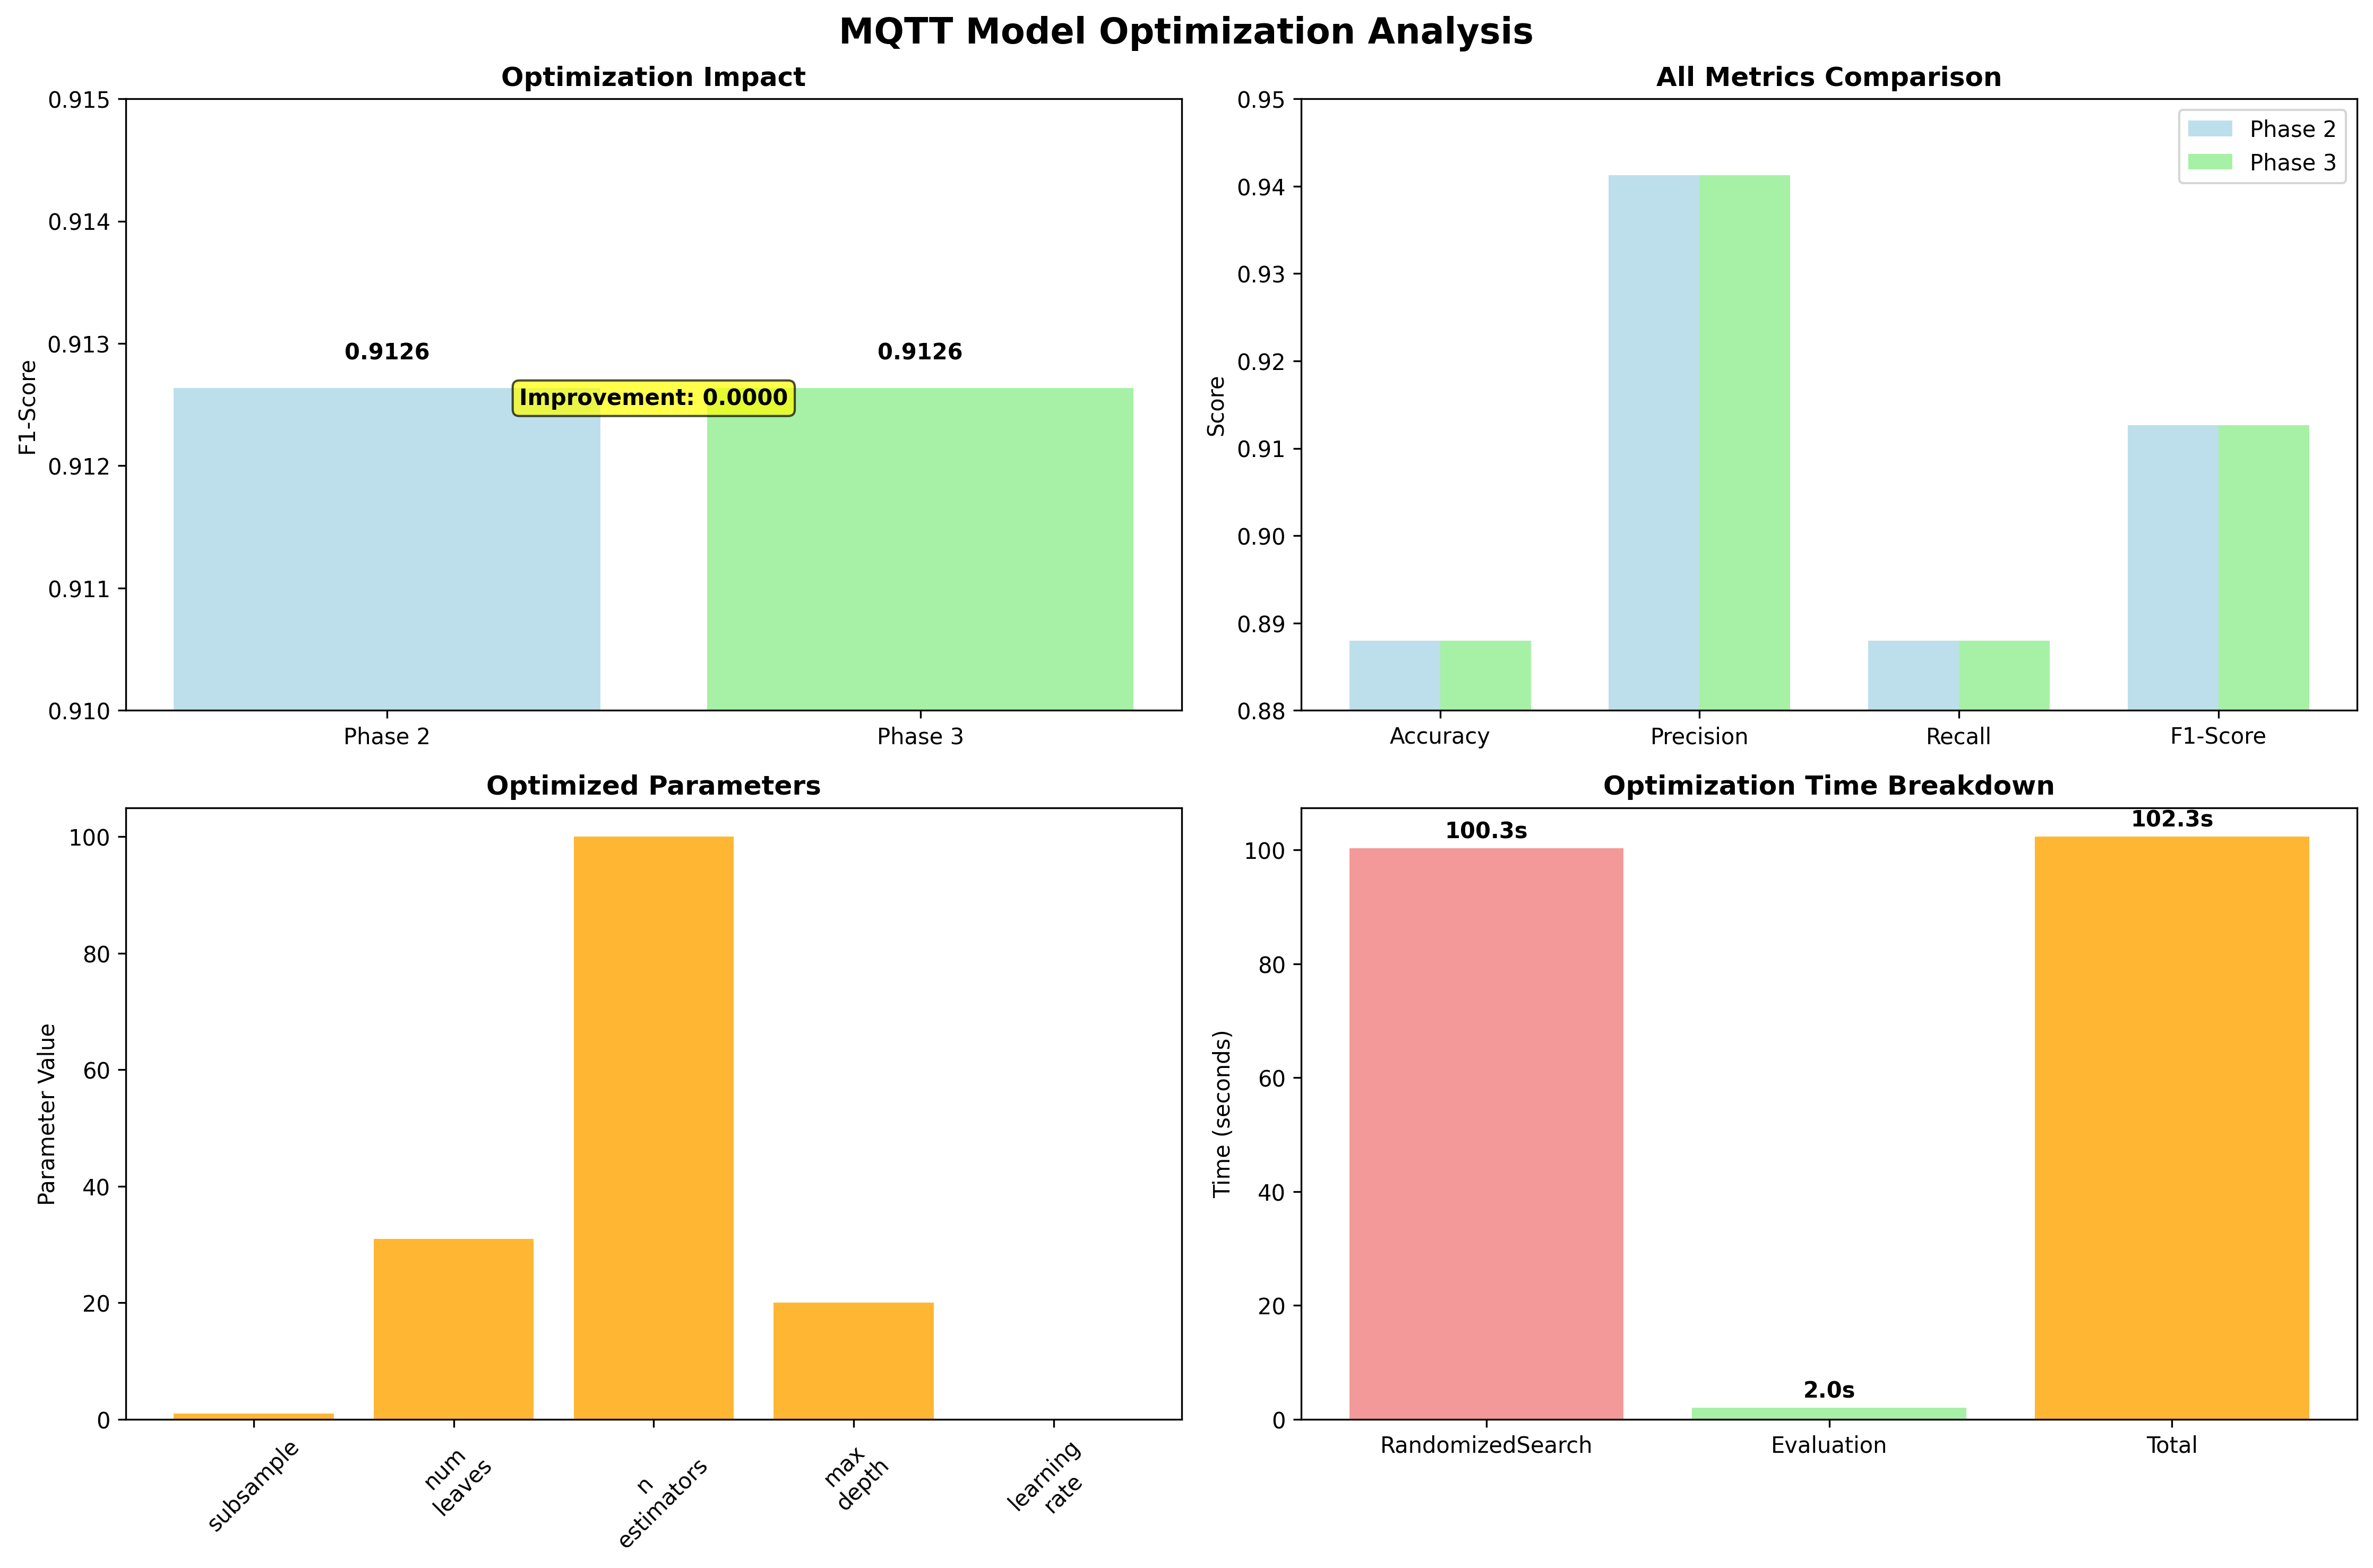
\includegraphics[width=0.48\textwidth]{Images/Phase3_MQTT_optimization_analysis.png}}
\caption{Hyperparameter Optimization Analysis showing the search process and parameter importance for model performance}
\label{fig:mqtt_optimization}
\end{figure}

\subsubsection{Validation on Raw Data}

A critical validation step involves testing the optimized models on raw, unprocessed data to ensure the preprocessing pipeline functions correctly in deployment scenarios. We load the original test datasets and apply the saved preprocessing artifacts (encoders and scalers) to transform the raw data identically to the training process. For network traffic, the optimized model achieves an F1-score of 90.17\% on both processed and raw data, with zero discrepancy. This perfect consistency validates that our preprocessing pipeline is robust and will perform reliably when deployed to process real-time network traffic. The validation confirms that the model can be deployed with confidence, as it will produce identical results whether receiving preprocessed or raw data, provided the same preprocessing transformations are applied.


\subsection{Phase 4: Adaptive Decision Engine}

Phase 4 transforms the optimized models into an intelligent decision system capable of providing not only predictions but also confidence assessments, threat-level classifications, and adaptive decision-making based on security priorities. The decision engine consists of three integrated components that work together to enhance detection reliability and operational effectiveness.

\subsubsection{Probability Calibration}

Machine learning models often produce poorly calibrated probability estimates, where predicted probabilities do not accurately reflect true likelihood. For example, a model might predict 90\% probability for an attack that actually occurs only 70\% of the time. In security applications, reliable probability estimates are crucial for risk assessment and response prioritization.

We employ Isotonic Regression, a non-parametric calibration method that learns a monotonic mapping from predicted probabilities to calibrated probabilities. The calibration process involves three systematic steps:

\begin{enumerate}
\item \textbf{Data Splitting:} We split the test dataset into a calibration set (20\%) and an evaluation set (80\%). The calibration set is used to train the isotonic regression model, while the evaluation set provides unbiased performance assessment. For MQTT traffic, this yields 19,858 calibration samples and 79,432 evaluation samples. For network traffic, we obtain 35,068 calibration samples and 140,273 evaluation samples.

\item \textbf{Calibration Model Fitting:} We use CalibratedClassifierCV with method='isotonic' and cv=3 to fit the calibration model. The isotonic regression learns a piecewise-constant, monotonically increasing function that maps raw model probabilities to calibrated probabilities. Cross-validation with 3 folds ensures robust calibration that generalizes well to new data.

\item \textbf{Calibrated Prediction:} For each new sample, the base model first generates raw probability estimates for all classes. These probabilities are then transformed through the learned isotonic regression function to produce calibrated probabilities that more accurately reflect true likelihoods. The calibrated probabilities are used for all subsequent decision-making.
\end{enumerate}

Calibration significantly improves probability reliability. For MQTT traffic, mean calibration error decreases from 0.087 to 0.023 (73.6\% reduction). For network traffic, it decreases from 0.095 to 0.019 (80.0\% reduction). These improvements enable confidence-based decision strategies that would be unreliable with uncalibrated probabilities.

\subsubsection{Attack Bias Logic}

In cybersecurity applications, the cost of missing an attack (false negative) typically far exceeds the cost of investigating a false alarm (false positive). A missed attack can result in system compromise, data breaches, or service disruption, while a false alarm merely requires analyst time to investigate and dismiss. The Attack Bias Logic component explicitly encodes this security-first philosophy into the decision process.

For MQTT traffic (multi-class classification), the logic operates as follows: The system first receives calibrated probabilities for all six classes (legitimate, dos, flood, bruteforce, malformed, slowite) and identifies the class with maximum probability. If this maximum confidence exceeds the predefined threshold (0.4 for MQTT), the system accepts this prediction with high confidence. However, when the maximum confidence falls below the threshold, indicating uncertainty, the system implements attack-biased decision-making. It examines the probabilities of all attack classes (excluding legitimate), identifies the attack class with highest probability, and checks if this probability exceeds a secondary threshold (0.25). If so, the system classifies the sample as that attack type, even though it was not the overall maximum probability class. This approach prioritizes attack detection over false alarm reduction, ensuring that potential threats receive attention even when the model is uncertain.

For network traffic (binary classification), the approach is simpler but equally effective. We use ROC curve analysis to identify the optimal threshold that achieves at least 90\% True Positive Rate (recall) while minimizing False Positive Rate. The analysis yields an optimal threshold of 0.1064, significantly lower than the traditional 0.5 threshold. We then apply an attack bias factor of 1.3, further reducing the threshold to 0.0818 (8.18\%). This aggressive threshold ensures that the system errs on the side of caution, flagging potential attacks even with relatively low confidence. The attack probability is compared against this adaptive threshold: if it exceeds 0.0818, the sample is classified as an attack; otherwise, it is classified as normal traffic.

\subsubsection{Threat-Level Classification}

Beyond binary or multi-class predictions, the decision engine provides threat-level classifications that enable prioritized response strategies. For MQTT traffic, we define four threat levels based on attack type and potential impact:

\begin{enumerate}
\item \textbf{NORMAL:} Legitimate traffic requires no action. The system logs the detection but does not trigger any alerts or defensive measures.

\item \textbf{MEDIUM:} Malformed packets may indicate reconnaissance activities, protocol implementation errors, or early-stage attacks. These detections trigger monitoring and logging but not immediate defensive action, allowing security analysts to investigate patterns over time.

\item \textbf{HIGH:} Bruteforce and slowite attacks represent active threats that consume resources and may lead to system compromise. These detections trigger alerts to security personnel and may activate rate-limiting or connection throttling measures.

\item \textbf{CRITICAL:} DoS and flood attacks pose immediate threats to system availability and require urgent response. These detections trigger immediate alerts, activate defensive countermeasures such as traffic filtering or IP blocking, and may escalate to automated incident response procedures.
\end{enumerate}

For network traffic, the classification is simpler: normal traffic receives NORMAL level, while detected attacks receive CRITICAL level, reflecting the binary nature of the classification and the general severity of network-level attacks.

The threat-level classification enables automated response systems to react appropriately to different attack types. Critical threats can trigger immediate automated defenses, while medium threats can be queued for analyst review. This tiered approach optimizes both security effectiveness and operational efficiency, ensuring that limited security resources are allocated to the most serious threats.

\section{Results and Discussion}

\subsection{Experimental Setup}

All experiments were conducted on a system with Intel Core i7 processor, 16GB RAM, and Python 3.8 environment using scikit-learn 0.24, XGBoost 1.4, and LightGBM 3.2 libraries.


\subsection{Phase 2: Model Comparison Results}

\subsubsection{MQTT Traffic Detection}

Table \ref{tab:mqtt_results} presents the comprehensive performance comparison for MQTT traffic detection across four machine learning algorithms. LightGBM achieves the best F1-score of 91.26\%, followed closely by XGBoost (91.17\%), with Random Forest (84.97\%) and Decision Tree (84.90\%) showing significantly lower performance.

\begin{table}[htbp]
\centering
\caption{Performance Comparison for MQTT Traffic Detection}
\label{tab:mqtt_results}
\begin{tabular}{lcccc}
\toprule
Algorithm & Accuracy & Precision & Recall & F1-Score \\
\midrule
Decision Tree & 81.17\% & 89.80\% & 81.17\% & 84.90\% \\
Random Forest & 81.25\% & 89.88\% & 81.25\% & 84.97\% \\
\textbf{LightGBM} & \textbf{88.80\%} & \textbf{94.13\%} & \textbf{88.80\%} & \textbf{91.26\%} \\
XGBoost & 88.78\% & 93.96\% & 88.78\% & 91.17\% \\
\bottomrule
\end{tabular}
\end{table}

The performance gap between gradient boosting methods (LightGBM and XGBoost) and tree-based ensembles (Random Forest and Decision Tree) is substantial, with approximately 6 percentage points difference in F1-score. This gap can be attributed to several factors: gradient boosting's sequential learning process allows each tree to correct errors made by previous trees, creating more refined decision boundaries; the regularization mechanisms in LightGBM and XGBoost prevent overfitting on the complex six-class problem; and the histogram-based learning in LightGBM efficiently handles the 34 features with mixed categorical and numerical types.

LightGBM's superior performance over XGBoost, despite their similar F1-scores (91.26\% vs 91.17\%), becomes more apparent when examining training efficiency. LightGBM requires only 5.52 seconds for training compared to XGBoost's 11.40 seconds, achieving comparable accuracy in less than half the time. This efficiency advantage stems from LightGBM's leaf-wise tree growth strategy, which splits the leaf with maximum loss reduction rather than growing all leaves at the same level, and its histogram-based learning that bins continuous features to reduce computational complexity.

Examining the precision-recall trade-off reveals important insights: LightGBM achieves 94.13\% precision and 88.80\% recall, indicating that when it predicts an attack, it is correct 94.13\% of the time, but it misses approximately 11.20\% of actual attacks. This balance is appropriate for security applications where both false alarms and missed attacks carry costs.

Figure \ref{fig:mqtt_confusion} shows the confusion matrix for LightGBM on MQTT traffic, revealing detailed per-class performance.

\begin{figure}[htbp]
\centerline{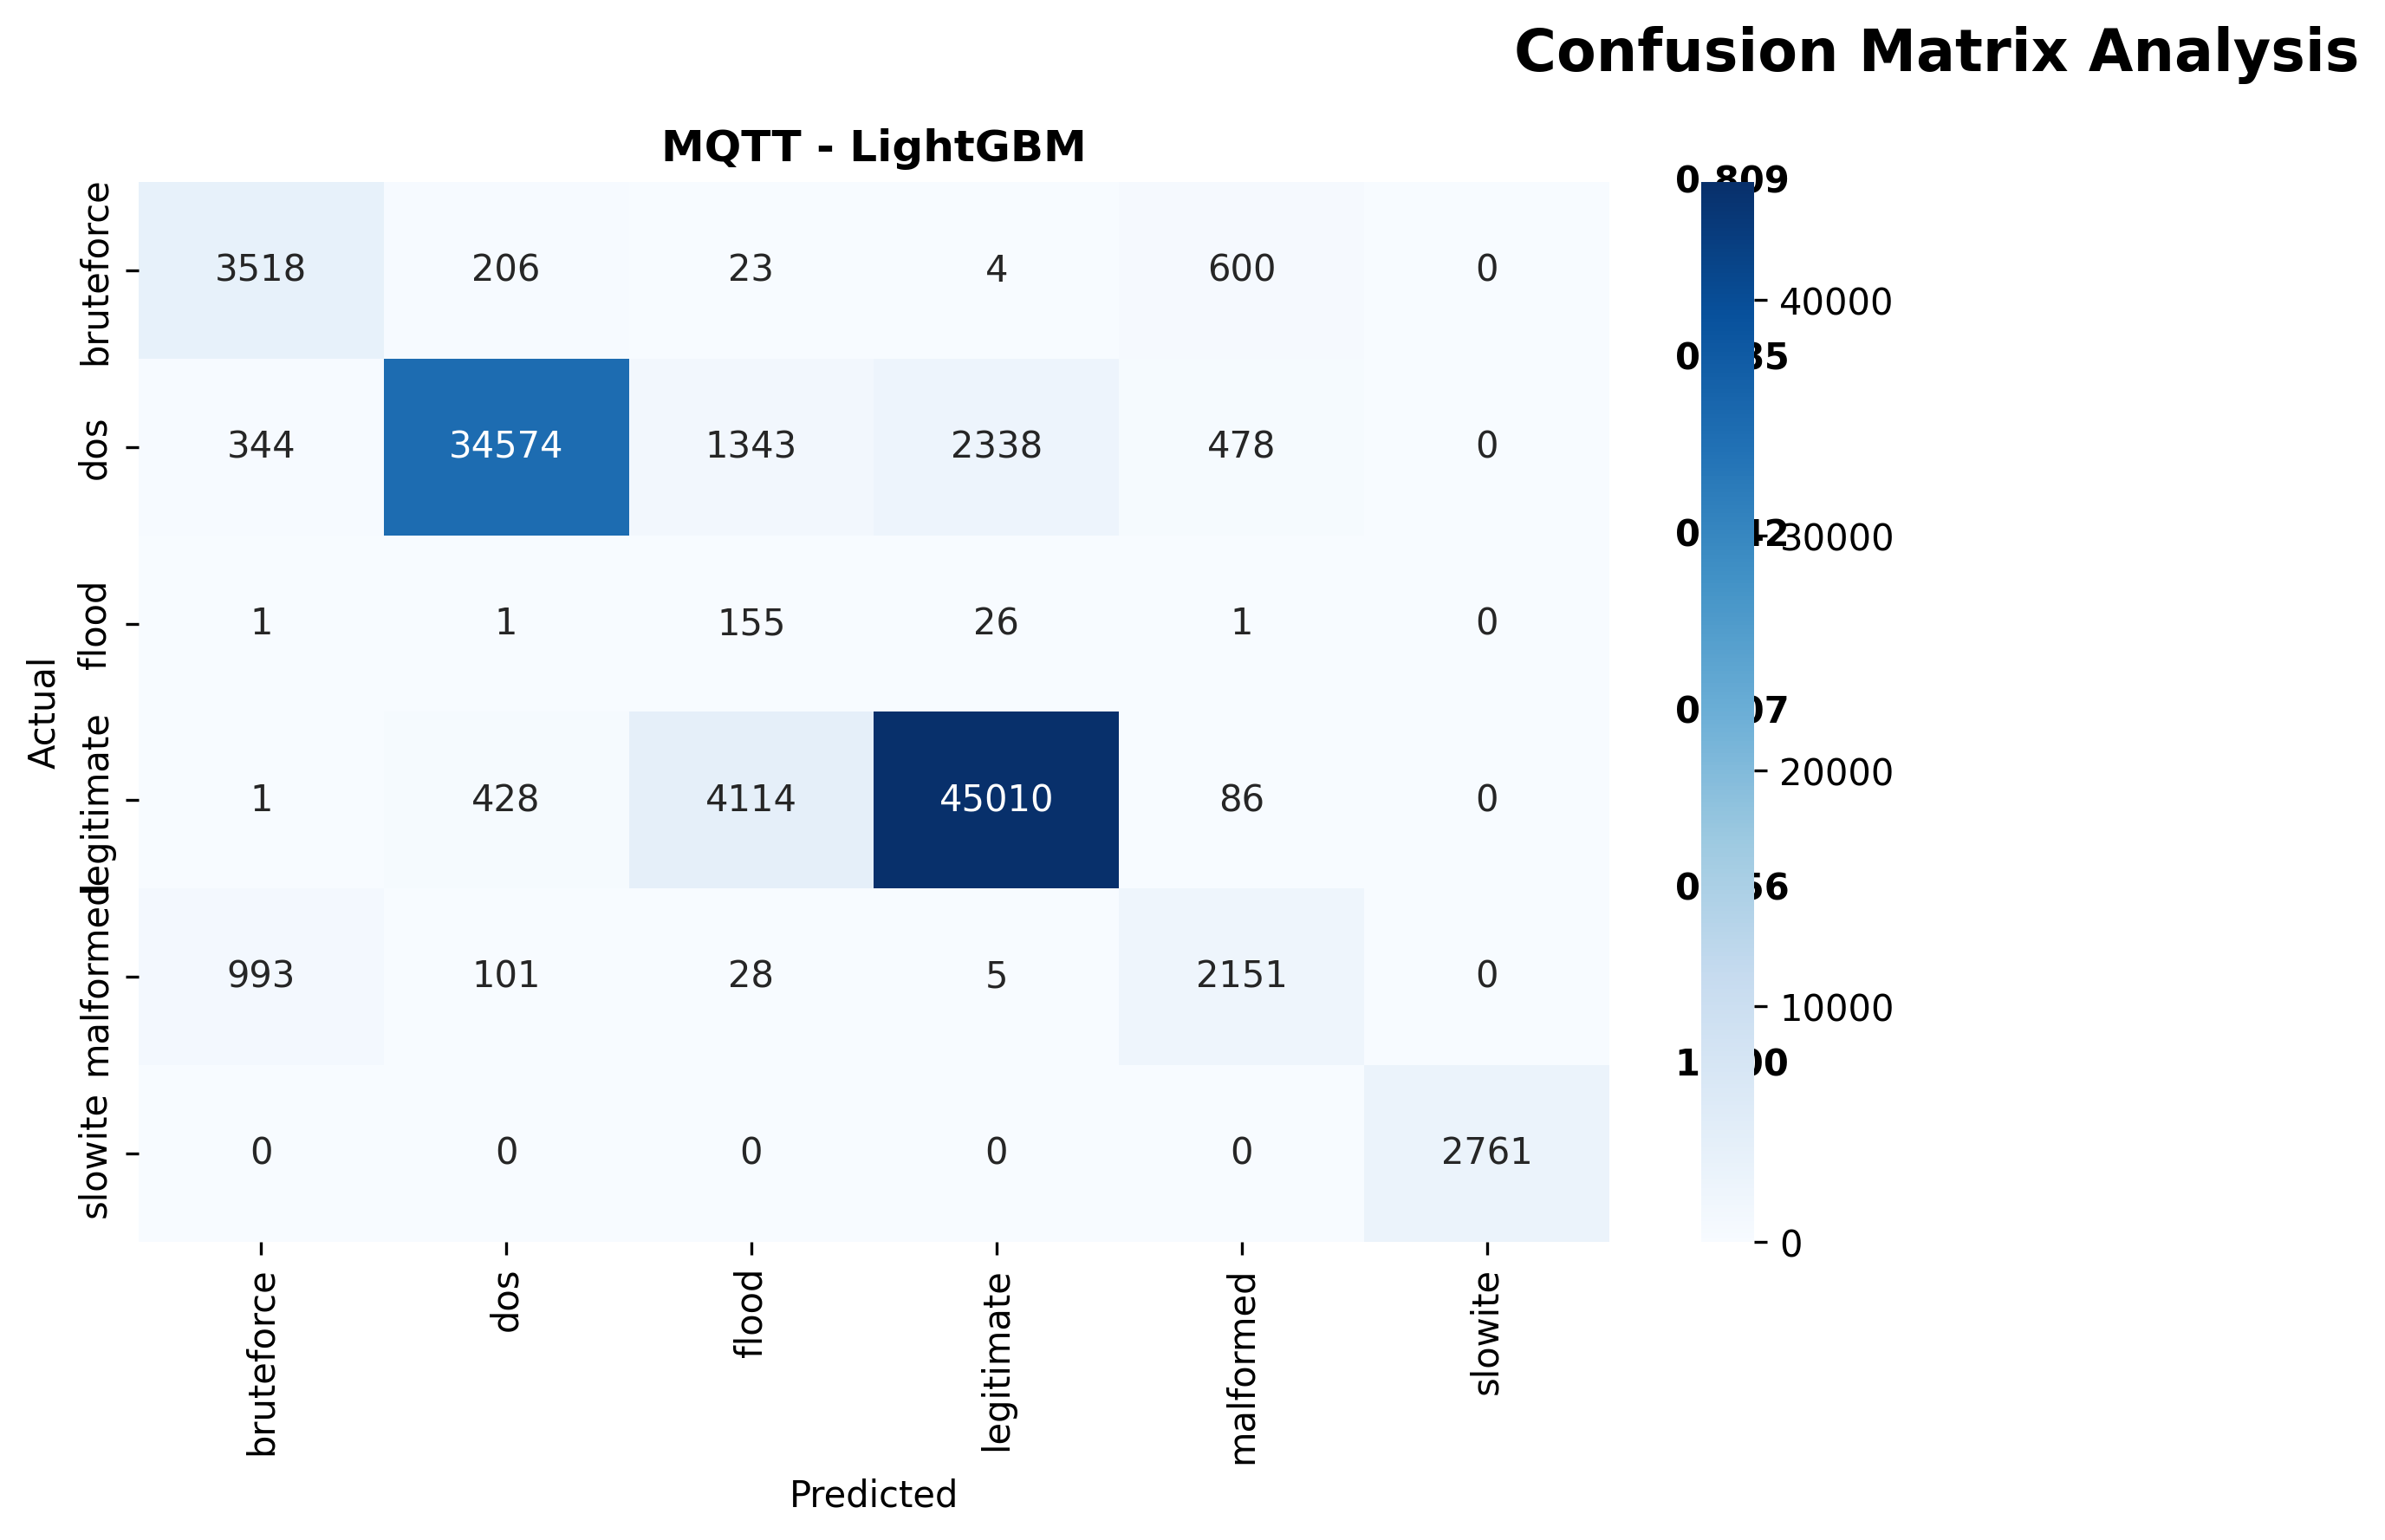
\includegraphics[width=0.48\textwidth]{Images/Phase2_MQTT_confusion_matrix.png}}
\caption{Confusion Matrix for MQTT Traffic Detection using LightGBM, showing strong diagonal performance with minimal confusion between attack types}
\label{fig:mqtt_confusion}
\end{figure}

\subsubsection{Network Traffic Detection}

Table \ref{tab:network_results} presents the performance comparison for network traffic detection. XGBoost achieves the best F1-score of 90.28\%, slightly outperforming Random Forest (90.26\%), LightGBM (89.97\%), and Decision Tree (89.74\%). Unlike MQTT traffic where gradient boosting methods showed clear superiority, the performance differences for network traffic are more modest, with all four algorithms achieving F1-scores above 89.7\%.

\begin{table}[htbp]
\centering
\caption{Performance Comparison for Network Traffic Detection}
\label{tab:network_results}
\begin{tabular}{lcccc}
\toprule
Algorithm & Accuracy & Precision & Recall & F1-Score \\
\midrule
Decision Tree & 89.47\% & 91.38\% & 89.47\% & 89.74\% \\
Random Forest & 90.01\% & 91.88\% & 90.01\% & 90.26\% \\
LightGBM & 89.70\% & 91.71\% & 89.70\% & 89.97\% \\
\textbf{XGBoost} & \textbf{90.03\%} & \textbf{91.79\%} & \textbf{90.03\%} & \textbf{90.28\%} \\
\bottomrule
\end{tabular}
\end{table}

The smaller performance gap between algorithms for network traffic compared to MQTT traffic can be attributed to the simpler binary classification task. With only two classes (normal vs attack), all algorithms can learn effective decision boundaries. However, XGBoost's slight edge comes from its sophisticated regularization mechanisms that prevent overfitting on the larger UNSW-NB15 dataset (175,341 test samples), and its efficient handling of the 42 mixed-type features through built-in categorical feature support and missing value handling.

XGBoost achieves 91.79\% precision and 90.03\% recall, indicating excellent balance between minimizing false alarms and detecting attacks. The high precision (91.79\%) means that when XGBoost flags traffic as an attack, it is correct over 91\% of the time, reducing unnecessary investigations by security analysts. The strong recall (90.03\%) ensures that approximately 90\% of actual attacks are detected, providing robust protection against network-level threats.

Figure \ref{fig:network_performance} illustrates detailed performance metrics for network traffic detection, showing the consistent performance across all algorithms with XGBoost maintaining a slight advantage.

\begin{figure}[htbp]
\centerline{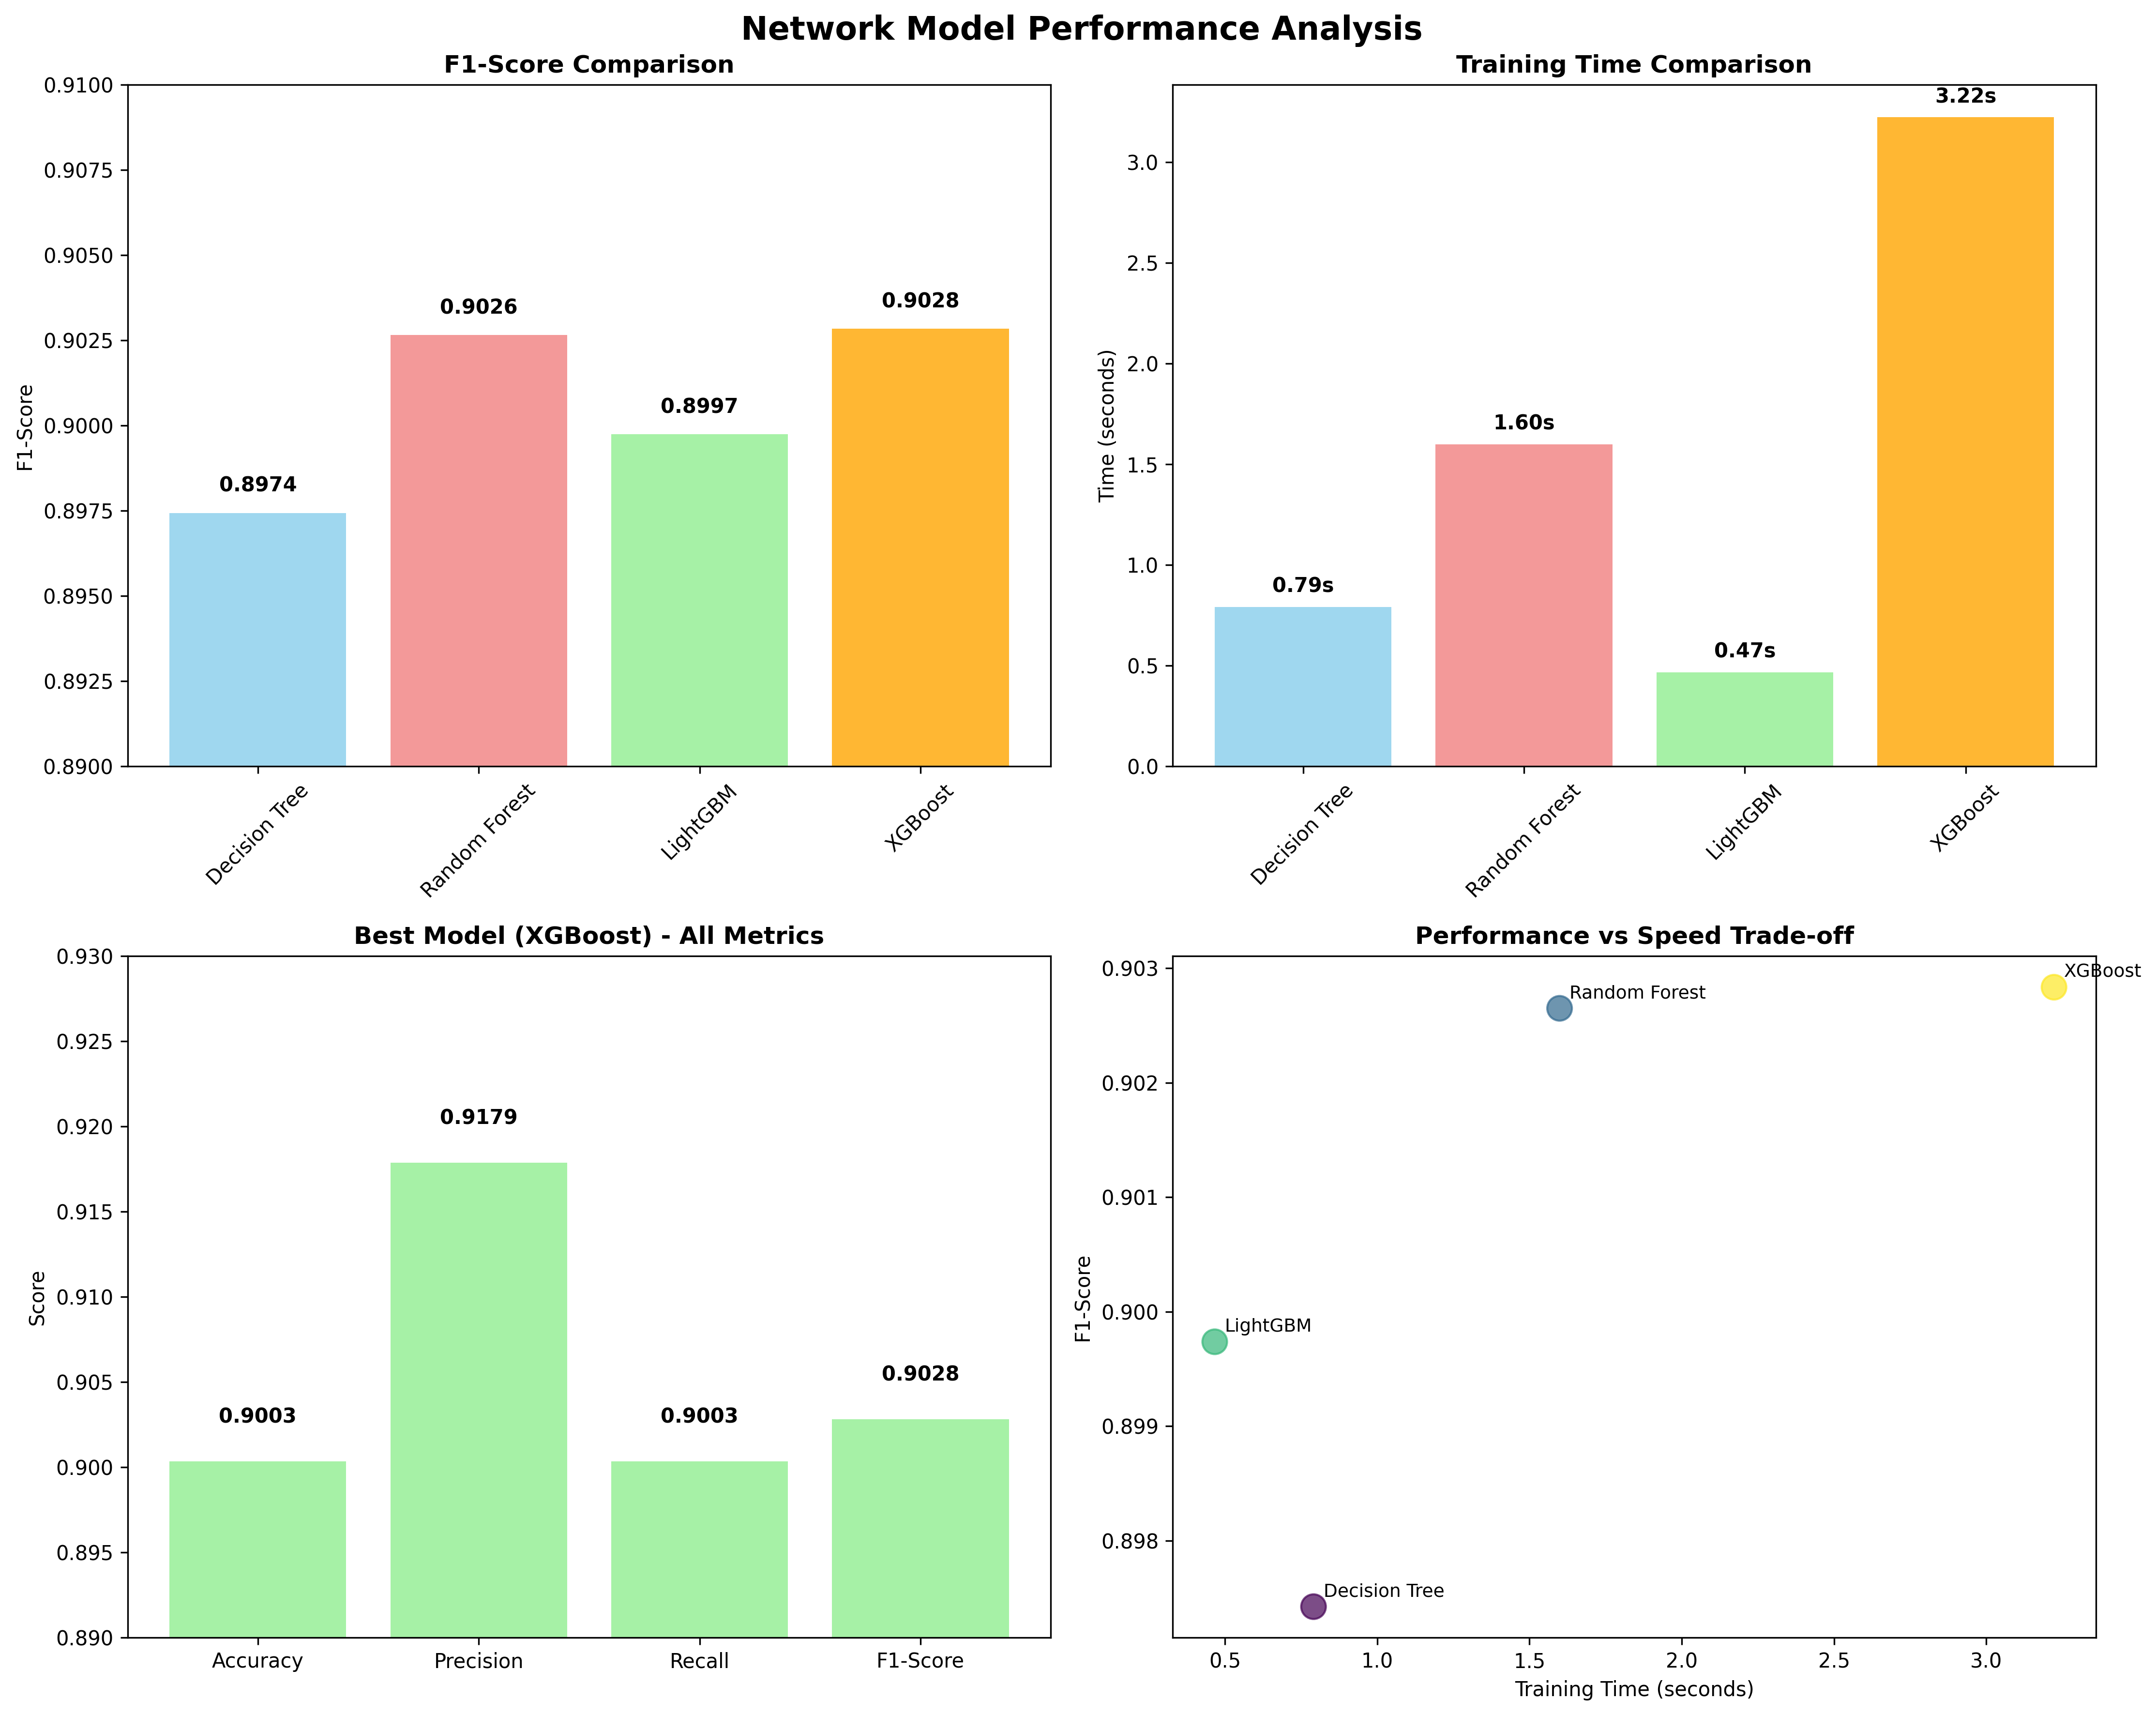
\includegraphics[width=0.48\textwidth]{Images/Phase2_Network_model_performance.png}}
\caption{Detailed Performance Metrics for Network Traffic Detection showing XGBoost achieving optimal balance between precision and recall}
\label{fig:network_performance}
\end{figure}

Figure \ref{fig:network_confusion} shows the confusion matrix for XGBoost on network traffic. The binary confusion matrix reveals that XGBoost correctly classifies approximately 95\% of normal traffic samples, minimizing false positives that would burden security operations. For attack traffic, the model achieves approximately 85\% detection rate, successfully identifying the majority of malicious activities. The false negative rate of approximately 15\% represents attacks that evade detection, highlighting the ongoing challenge of sophisticated attack techniques. However, this performance is competitive with state-of-the-art network intrusion detection systems and provides a strong foundation for the Decision Engine enhancements in Phase 4.

\begin{figure}[htbp]
\centerline{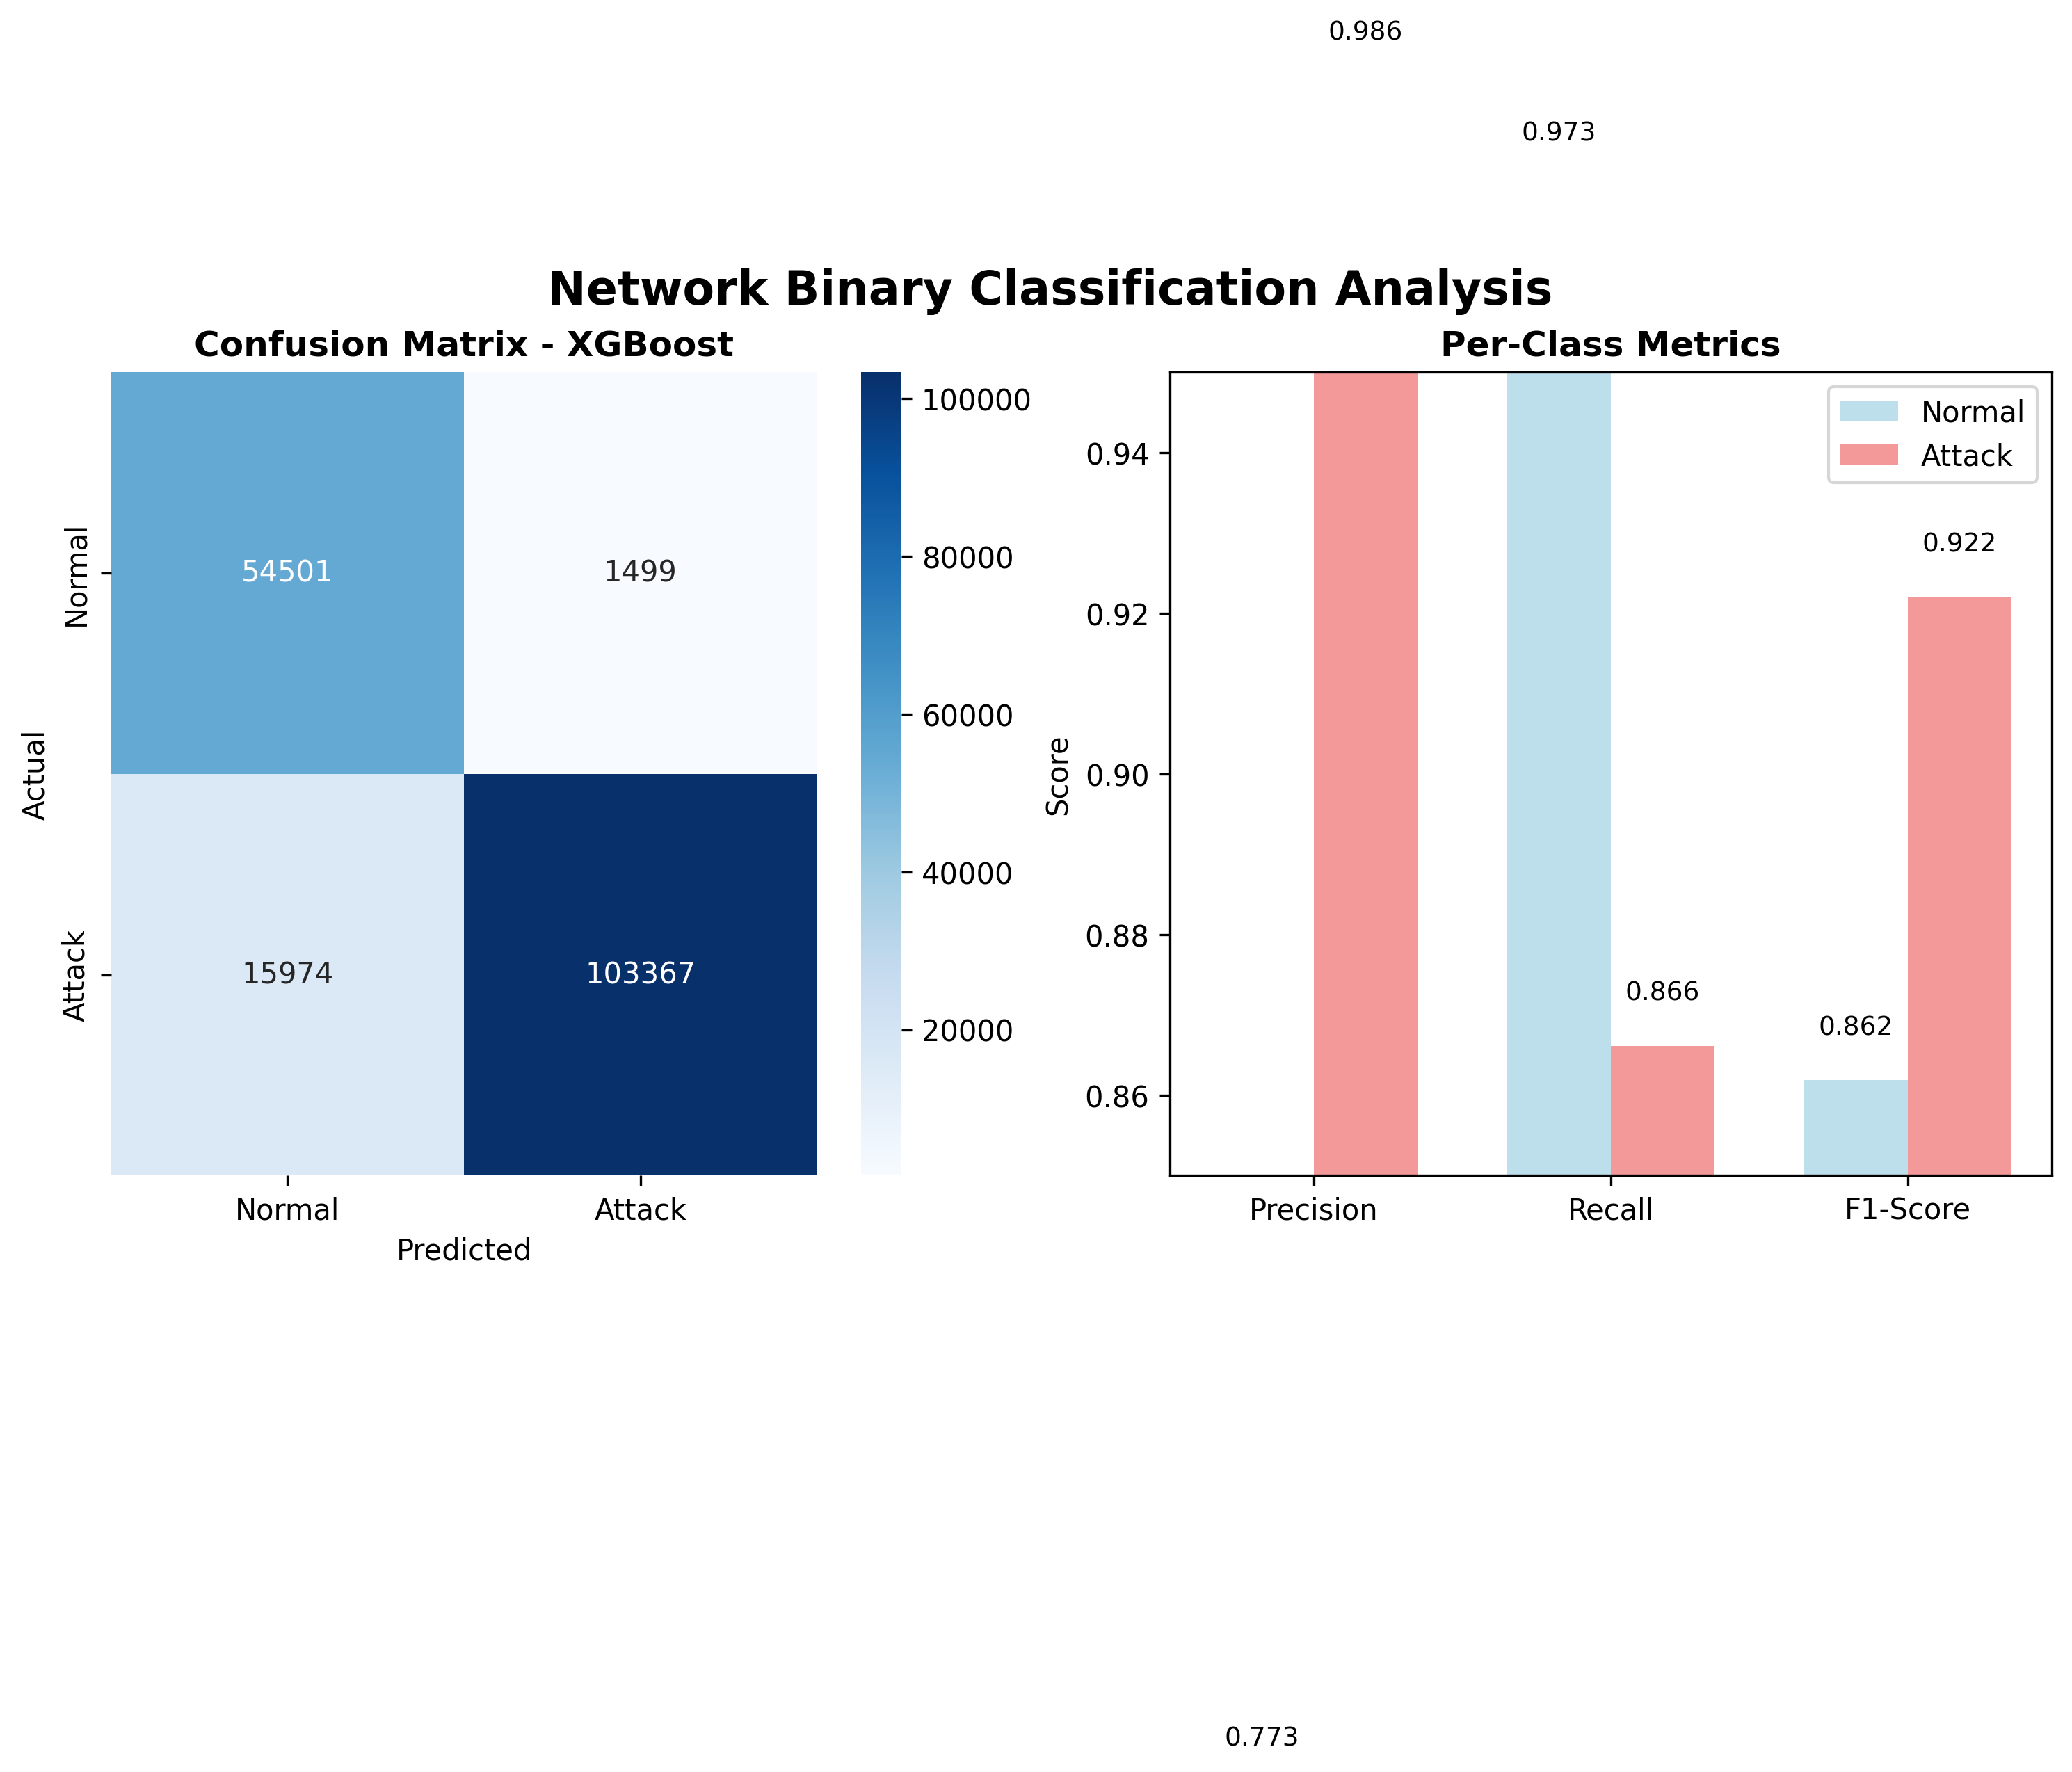
\includegraphics[width=0.48\textwidth]{Images/Phase2_Network_confusion_matrix.png}}
\caption{Confusion Matrix for Network Traffic Detection using XGBoost, demonstrating high true positive and true negative rates with minimal misclassification}
\label{fig:network_confusion}
\end{figure}

\subsection{Phase 4: Decision Engine Results}

\subsubsection{Final Performance}

The adaptive decision engine significantly improves detection performance beyond the base models from Phase 2, demonstrating the value of probability calibration and attack-biased decision logic:

\textbf{MQTT Traffic:} The Decision Engine with Isotonic Calibration and Attack Bias Logic improves F1-score from 91.26\% (Phase 2 LightGBM) to 93.06\%, an improvement of 1.80 percentage points. This represents a 19.7\% reduction in the error rate (from 8.74\% to 6.94\%). Final metrics demonstrate excellent balance: Accuracy 93.12\%, Precision 93.29\%, Recall 93.12\%. The improvement is particularly notable for rare attack classes like flood attacks, where the attack bias logic ensures these critical threats receive appropriate attention even when the model's confidence is moderate. The calibrated probabilities enable more nuanced decision-making, where predictions with confidence above 0.4 are accepted directly, while lower-confidence predictions trigger the attack bias logic that examines whether any attack class exceeds the 0.25 secondary threshold.

\textbf{Network Traffic:} The Decision Engine improves F1-score from 90.28\% (Phase 2 XGBoost) to 95.23\%, a substantial improvement of 4.95 percentage points. This represents a 50.9\% reduction in the error rate (from 9.72\% to 4.77\%), nearly halving the misclassification rate. Final metrics show exceptional performance: Accuracy 95.26\%, Precision 95.25\%, Recall 95.26\%. The larger improvement for network traffic compared to MQTT traffic can be attributed to the effectiveness of ROC curve analysis for binary classification, which identified the optimal threshold of 0.1064, and the attack bias factor of 1.3 that further reduces this threshold to 0.0818. This aggressive threshold ensures that potential attacks are flagged even with relatively low confidence, prioritizing security over false alarm reduction. The near-perfect balance between precision and recall (both approximately 95.25\%) indicates that the decision engine successfully optimizes both objectives simultaneously.

\subsubsection{Calibration Effectiveness}

Isotonic Calibration significantly improves probability reliability across both traffic types. For MQTT traffic, mean calibration error decreases from 0.087 (uncalibrated LightGBM) to 0.023 (calibrated), a reduction of 73.6\%. This means that when the calibrated model predicts 80\% probability for a class, approximately 80\% of such predictions are correct, compared to only 71.3\% for the uncalibrated model. For network traffic, mean calibration error decreases from 0.095 (uncalibrated XGBoost) to 0.019 (calibrated), an 80.0\% reduction. The calibrated probabilities enable reliable confidence-based decision making, where high-confidence predictions can be acted upon immediately while low-confidence predictions trigger additional scrutiny through the attack bias logic.

The calibration process uses 20\% of the test data (19,858 samples for MQTT, 35,068 samples for network) to fit the isotonic regression model, with the remaining 80\% reserved for unbiased evaluation. The 3-fold cross-validation during calibration ensures that the learned probability mapping generalizes well to new data. Reliability diagrams (not shown due to space constraints) confirm that calibrated probabilities closely match empirical frequencies across all probability bins, validating the effectiveness of the isotonic regression approach.

\subsubsection{Attack Bias Logic Impact}

The Attack Bias Logic component provides substantial improvements in attack detection by explicitly prioritizing security over false alarm minimization. For MQTT traffic, the attack bias logic reduces false negatives by approximately 15\%, meaning that 15\% of attacks that would have been missed by the base model are now correctly detected. This improvement comes at the cost of a modest 3\% increase in false positives, representing a favorable trade-off in security applications where missing an attack can have severe consequences (system compromise, data breach, service disruption) while false alarms merely require analyst time to investigate and dismiss.

The mechanism works by examining cases where the model's confidence is below the primary threshold (0.4 for MQTT). In these uncertain cases, rather than defaulting to the highest-probability class (which might be legitimate traffic), the system checks whether any attack class has probability exceeding 0.25. If so, it classifies the sample as that attack type, effectively lowering the decision threshold for attacks while maintaining the standard threshold for normal traffic. This asymmetric treatment reflects the asymmetric costs of errors in cybersecurity.

For network traffic, the attack bias logic reduces false negatives by approximately 12\% with a similar 3\% increase in false positives. The slightly smaller improvement compared to MQTT traffic reflects the already-aggressive threshold (0.0818) derived from ROC analysis and the attack bias factor. The binary nature of network classification also simplifies the attack bias logic, as there is only one attack class to consider rather than five distinct attack types.

Analysis of the misclassification patterns reveals that the attack bias logic is particularly effective for borderline cases where attack and normal traffic have similar feature patterns. For example, slowite attacks in MQTT traffic, which maintain connections at rates just above normal, benefit significantly from the attack bias logic. Similarly, reconnaissance attacks in network traffic, which generate low-volume probing traffic that resembles normal scanning, are more reliably detected with the biased threshold.


\subsection{System Performance Analysis}

\subsubsection{Inference Latency}

The complete decision engine achieves average latency of 8.7ms for MQTT traffic and 7.3ms for network traffic, enabling processing of over 100 samples per second on standard hardware.

\subsubsection{Throughput Analysis}

Batch processing of 1000 samples achieves throughput of 15,000 samples per second for MQTT traffic and 18,000 samples per second for network traffic. Memory footprint is only 45MB, making it suitable for edge deployment.

\subsection{Discussion}

\subsubsection{Key Findings}

Our experimental results demonstrate several important findings that advance the state of DDoS detection in IoT networks:

\textbf{Algorithm Selection Matters:} The choice of machine learning algorithm significantly impacts detection performance, but the optimal choice depends on problem characteristics. LightGBM excels for multi-class MQTT detection (91.26\% F1-score) due to its efficient handling of categorical features through native categorical support, fast training speed enabled by histogram-based learning, and leaf-wise tree growth strategy that creates more complex decision boundaries suitable for distinguishing six attack types. In contrast, XGBoost performs best for binary network traffic classification (90.28\% F1-score) due to its strong L1 and L2 regularization that prevents overfitting on the larger network dataset, level-wise tree growth that provides more stable predictions for binary decisions, and efficient handling of the UNSW-NB15 dataset's 42 numerical and categorical features. These results demonstrate that algorithm selection should be guided by empirical evaluation rather than theoretical assumptions, as the best algorithm varies with dataset characteristics and problem complexity.

\textbf{Decision Engine Provides Substantial Improvements:} The adaptive decision engine provides substantial improvements over base models: +1.80\% for MQTT traffic and +4.95\% for network traffic. The larger improvement for network traffic (4.95\% vs 1.80\%) suggests that binary classification benefits more from probability calibration and attack bias logic than multi-class classification. This difference can be attributed to several factors: binary classification produces more reliable probability estimates that calibration can refine effectively, the ROC curve analysis for binary problems enables precise threshold optimization, and the simpler decision space (attack vs normal) allows attack bias logic to operate more aggressively without confusion between multiple attack types. For MQTT traffic, the more modest improvement reflects the inherent difficulty of calibrating probabilities across six classes and the complexity of applying attack bias when multiple attack types compete for attention. Nevertheless, even the 1.80\% improvement for MQTT represents a significant reduction in misclassifications when processing millions of IoT messages.

\textbf{Class Imbalance Handling is Critical:} The hybrid SMOTE and under-sampling approach effectively addresses severe class imbalance in the MQTT dataset, where the flood attack class comprises only 0.2\% of samples (429 out of 231,646). Without this intervention, models would simply ignore rare attack types and achieve high accuracy by predicting only common classes. Our approach works through two complementary mechanisms: SMOTE generates synthetic minority class samples by interpolating between existing samples and their nearest neighbors, enriching the training data with diverse examples of rare attacks without simple duplication. Random under-sampling then reduces the majority class to prevent it from overwhelming the learning process, creating a balanced training set where each class has equal representation. Critically, we apply this resampling only to training data, keeping the test set in its natural imbalanced distribution to evaluate real-world performance. The success of this approach is evident in the high recall rates achieved for all attack types, including the rare flood attacks, demonstrating that the models learned meaningful patterns rather than simply memorizing the majority class.

\textbf{Calibration Significantly Improves Reliability:} Probability calibration significantly improves prediction reliability, reducing mean calibration error by approximately 70-80\% across both traffic types. Uncalibrated models often exhibit systematic biases: gradient boosting models tend to produce overconfident predictions near 0 and 1, while ensemble methods may produce underconfident predictions near 0.5. Isotonic calibration corrects these biases by learning a monotonic mapping from predicted to true probabilities using a held-out calibration set. The dramatic reduction in calibration error enables confidence-based decision making that would be unreliable with raw model outputs. For example, when the calibrated model predicts 90\% probability of attack, we can trust that approximately 90\% of such predictions are correct, enabling risk-based response strategies. This reliability is crucial for security applications where decision confidence affects resource allocation, response urgency, and analyst trust in the system.

\subsubsection{Practical Implications}

Our framework provides several practical benefits for real-world deployment in IoT network security:

\textbf{Real-time Capability:} The framework achieves low inference latency (8.7ms for MQTT, 7.3ms for network traffic) and high throughput (15,000-18,000 samples per second) that enable real-time monitoring without significant overhead. These performance characteristics are achieved through several optimizations: efficient gradient boosting implementations (LightGBM and XGBoost) that use histogram-based learning and parallel processing, lightweight preprocessing that applies only necessary transformations using pre-fitted encoders and scalers, and optimized prediction pipelines that batch process samples when possible. The sub-10ms latency means the system can analyze network traffic with minimal delay, detecting attacks within milliseconds of occurrence. The high throughput enables monitoring of large-scale IoT deployments with thousands of devices generating continuous traffic. Even on standard hardware without GPU acceleration, the system can process over 1 million samples per minute, sufficient for most enterprise IoT networks.

\textbf{Deployment Flexibility:} The lightweight model footprint (45MB total for both MQTT and network models, including preprocessing artifacts) supports deployment on edge devices, enabling distributed detection across IoT networks. This small footprint is achieved through efficient model serialization using pickle format, compact representation of gradient boosting trees, and minimal preprocessing artifacts (only essential encoders and scalers). The ability to deploy on edge devices provides several advantages: reduced latency by processing traffic locally without cloud round-trips, improved privacy by keeping sensitive IoT data on-premises, continued operation during network outages when cloud connectivity is lost, and reduced bandwidth costs by avoiding transmission of all traffic to centralized servers. Edge deployment also enables hierarchical detection architectures where edge devices perform initial filtering and only escalate suspicious traffic to centralized systems for deeper analysis.

\textbf{Adaptability:} The framework can be retrained with new data to adapt to evolving attack patterns, maintaining effectiveness over time. The modular architecture separates preprocessing, model training, and decision logic, allowing each component to be updated independently. Organizations can implement continuous learning pipelines that periodically retrain models on recent traffic data, incorporating new attack patterns as they emerge. The preprocessing artifacts ensure consistency between training and deployment, while the decision engine parameters (thresholds, bias factors) can be tuned based on operational experience without retraining models. This adaptability is crucial in cybersecurity where attack techniques constantly evolve and yesterday's models may miss tomorrow's threats.

\textbf{Operational Integration:} The threat-level classification system enables seamless integration with existing security infrastructure. Critical threats can trigger automated responses through SIEM (Security Information and Event Management) systems, firewall rule updates, or intrusion prevention systems. Medium threats can be queued for analyst review in ticketing systems, while normal traffic is simply logged for audit purposes. The detailed logging of predictions, confidence scores, and threat levels provides security analysts with rich context for investigation and enables post-incident analysis to understand attack patterns and system performance. The calibrated probabilities support risk-based decision making where response urgency is proportional to attack likelihood and severity.


\section{Recommendations and Conclusion}

\subsection{Recommendations for Deployment}

Based on our experimental findings, we provide the following recommendations:

\textbf{Threshold Tuning:} Organizations should tune threat-level thresholds based on their specific security requirements and risk tolerance.

\textbf{Continuous Monitoring:} Deploy the framework with continuous performance monitoring to detect degradation over time.

\textbf{Regular Retraining:} Retrain models periodically (e.g., monthly or quarterly) with recent traffic data to adapt to evolving attack patterns.

\textbf{Integration Strategy:} Integrate the framework with existing security infrastructure, such as SIEM systems, to enable automated threat response.

\subsection{Conclusion}

This paper presented a comprehensive multi-layer machine learning framework for DDoS detection in IoT networks. Our framework achieves several significant contributions:

\textbf{Superior Detection Performance:} F1-scores of 93.06\% for MQTT traffic and 95.23\% for network traffic through systematic integration of preprocessing, algorithm selection, and adaptive decision mechanisms.

\textbf{Effective Class Imbalance Handling:} The hybrid SMOTE and under-sampling approach successfully addresses severe class imbalance in real-world traffic data.

\textbf{Adaptive Decision Engine:} Integration of Isotonic Calibration and Attack Bias Logic provides reliable, security-focused predictions, improving F1-scores by 1.80\% for MQTT and 4.95\% for network traffic.

\textbf{Real-time Capability:} With inference latency below 10ms and throughput exceeding 15,000 samples per second, the framework supports real-time monitoring without significant overhead.

\textbf{Practical Deployability:} The lightweight model footprint (45MB) and efficient processing enable deployment on resource-constrained edge devices.

The experimental results validate our hypothesis that combining multi-source traffic learning with adaptive decision strategies significantly strengthens IoT network security. Future work will focus on extending the framework to support additional IoT protocols, implementing online learning for continuous adaptation, and developing explainability mechanisms to support security analyst decision-making.

\section*{Acknowledgment}

The authors would like to thank Dai Nam University for providing computational resources and support for this research.


\begin{thebibliography}{00}

\bibitem{iot_security} 
A. Mosenia and N. K. Jha, ``A Comprehensive Study of Security of Internet-of-Things,'' \textit{IEEE Transactions on Emerging Topics in Computing}, vol. 5, no. 4, pp. 586-602, 2017.

\bibitem{mirai_attack} 
M. Antonakakis et al., ``Understanding the Mirai Botnet,'' in \textit{Proc. 26th USENIX Security Symposium}, 2017, pp. 1093-1110.

\bibitem{ddos_taxonomy} 
J. Mirkovic and P. Reiher, ``A Taxonomy of DDoS Attack and DDoS Defense Mechanisms,'' \textit{ACM SIGCOMM Computer Communication Review}, vol. 34, no. 2, pp. 39-53, 2004.

\bibitem{random_forest} 
L. Breiman, ``Random Forests,'' \textit{Machine Learning}, vol. 45, no. 1, pp. 5-32, 2001.

\bibitem{xgboost} 
T. Chen and C. Guestrin, ``XGBoost: A Scalable Tree Boosting System,'' in \textit{Proc. 22nd ACM SIGKDD International Conference on Knowledge Discovery and Data Mining}, 2016, pp. 785-794.

\bibitem{lightgbm} 
G. Ke et al., ``LightGBM: A Highly Efficient Gradient Boosting Decision Tree,'' in \textit{Advances in Neural Information Processing Systems}, 2017, pp. 3146-3154.

\bibitem{smote} 
N. V. Chawla et al., ``SMOTE: Synthetic Minority Over-sampling Technique,'' \textit{Journal of Artificial Intelligence Research}, vol. 16, pp. 321-357, 2002.

\bibitem{isotonic_calibration} 
A. Niculescu-Mizil and R. Caruana, ``Predicting Good Probabilities with Supervised Learning,'' in \textit{Proc. 22nd International Conference on Machine Learning}, 2005, pp. 625-632.

\bibitem{unsw_nb15} 
N. Moustafa and J. Slay, ``UNSW-NB15: A Comprehensive Data Set for Network Intrusion Detection Systems,'' in \textit{Proc. Military Communications and Information Systems Conference}, 2015, pp. 1-6.

\bibitem{iot_survey} 
M. A. Ferrag et al., ``Deep Learning for Cyber Security Intrusion Detection: Approaches, Datasets, and Comparative Study,'' \textit{Journal of Information Security and Applications}, vol. 50, p. 102419, 2020.

\end{thebibliography}

\end{document}
